\documentclass[cfonts]{nostarch}

\usepackage{lipsum}
\hyphenation{ve-sti-bu-lum sene-c-tus rut-rum con-sec-te-tu-er
  elei-fend no-num-my li-be-ro}

\usepackage{natbib}
\usepackage{nshyper}
\lstset{fancyvrb=true}


% our additions to the preamble (make external)
%\usepackage[python]{runcode}
%\usepackage[python,stopserver]{runcode}
\usepackage[R]{runcodeBook}
%\usepackage[cache]{runcodeBook}

\usepackage{multirow}

%\usepackage{mdframed}
%\BeforeBeginEnvironment{minted}{\begin{mdframed}}
%\AfterEndEnvironment{minted}{\end{mdframed}}

\let\code\texttt
\let\proglang\textsf
\newcommand{\pkg}[1]{{\fontshape{it}\selectfont #1}}
\def\R{\textsf{R} }

% self defined environment and commands
\newcounter{example}% [section]
\newenvironment{example}[1][]{\refstepcounter{example}\par\medskip
   \noindent \textbf{Example~\theexample. (#1)} \rmfamily}{\medskip}
   % \noindent \textbf{Example~\thesection.\theexample. (#1)} \rmfamily}{\medskip}



\makeindex
\begin{document}


\frontmatter
\author{Haim~Bar, HaiYing~Wang, and Jun~Yan}

\title{Stumbling into data science}

\subtitle{A game-based introduction}

\nostarchlogo{images/nsp_logo_black_big.jpg}

\makehalftitle

\maketitle


\begin{copyrightpage}
  \textbf{\sffamily\MakeUppercase{Stumbling into Data Science.}}
  Copyright \textcopyright{} 2021 by
  Haim~Bar, HaiYing~Wang, and Jun~Yan
  
  All rights reserved. No part of this work may be reproduced or
  transmitted in any form or by any means, electronic or mechanical,
  including photocopying, recording, or by any information storage or
  retrieval system, without the prior written permission of the
  copyright owner and the publisher.

Printed in the United States of America

25 24 23 22 21 \hspace{0.5in}  1 2 3 4 5 6 7 8 9

ISBN-13: 123-4-5678-9012-3 (print)\\
ISBN-13: 123-4-5678-9012-3 (ebook)

Publisher: Bill Pollock\\
Production Manager: Rachel Monaghan\\
Production Editor: E.~D.~Itor\\
Developmental Editor: D.~E.~Itor\\
Cover Illustrator: Illustrator\\
Interior Design: Calamari Studios\\
Technical Reviewer: R.~E.~Viewer\\
Copyeditor: C.~O.~Editor\\
Proofreader: P.~R.~\O freader\\
Indexer: I.~N.~Dexer

For information on book distributors or translations, please contact
No Starch Press, Inc. directly: \\
No Starch Press, Inc.\\
245 8th Street, San Francisco, CA 94103\\
phone: 415.863.9900; fax: 415.863.9950; info@nostarch.com; www.nostarch.com\\

\begin{cipblock}
Uthor, A. U. and Respondent, C. O. R. and Iter, W. R.
  Pellentesque habitant morbi: Cum sociis natoque penatibus/
  A. U. Thor, C. O. R. Respondent and W. R. Iter
       p. cm.
  Includes index.
  ISBN-10: 1-23456-789-0
  ISBN-13: 123-4-56789-012-3
  1.  Morbi (habitant).  2. Penatibus. I. Title.
XX2303.5.T324 2008
\end{cipblock}

No Starch Press and the No Starch Press logo are registered trademarks
of No Starch Press, Inc. Other product and company names mentioned
herein may be the trademarks of their respective owners. Rather than
use a trademark symbol with every occurrence of a trademarked name, we
are using the names only in an editorial fashion and to the benefit of
the trademark owner, with no intention of infringement of the
trademark.

The information in this book is distributed on an ``As Is'' basis,
without warranty. While every precaution has been taken in the
preparation of this work, neither the author nor No Starch Press, Inc.
shall have any liability to any person or entity with respect to any
loss or damage caused or alleged to be caused directly or indirectly
by the information contained in it.

\vspace{0.7in}

[S]

\end{copyrightpage}

\begin{dedicationpage}
  Haim: To my family ... ...
  

  \bigskip

  HaiYing: To my family ... ...

  \bigskip

  Jun: To Jo, Bo, and Jiafeng, without whom the book would have been finished
  much sooner, but life would be unimaginable.
  
%   God of the golden bow,\\
%       And of the golden lyre,\\
% And of the golden hair,\\
%       And of the golden fire,\\
%             Charioteer\\
%             Of the patient year,\\
%       Where---where slept thine ire,\\
% When like a blank idiot I put on thy wreath,\\
%       Thy laurel, thy glory,\\
%       The light of thy story,\\
% Or was I a worm---too low crawling for death?\\
%       O Delphic Apollo!

% \bigskip
% \emph{John Keats}
% \index{Keats, John@\emph{Keats, John}}
% \index{gods!Greek!Apollo}
% \index{Apollo|see{gods, Greek}}
% \index{Greek gods|see{gods, Greek}}
\end{dedicationpage}

\newpage\null\thispagestyle{empty}\newpage

\null\vskip1.175in
\thispagestyle{empty}
\section*{About the Authors}
\textbf{Haim Bar} is an Associate Professor in the Department of Statistics,
University of Connecticut. Before joining UConn, he worked as a software
engineer for Motorola, a director of software development in MicroPatent, LLC, a
Principal Scientist at ATC-NY, and a statistician at Cornell's Statistical
Consulting Unit.
His research interests include Bayesian methods, statistical modeling and variable 
selection in high-dimensional data, especially in applications to genomics.


\noindent\textbf{HaiYing Wang} is an Associate Professor in the Department of
Statistics, University of Connecticut. He was an Assistant Professor in the
Department of Mathematics and Statistics at the University of New Hampshire and
an cooling system engineer in the Midea Group. His research interests include
informative subdata selection for big data, model selection, model averaging,
measurement error models, optimal design, and semi-parametric regression.

\noindent\textbf{Jun Yan} is a Professor in the Department of Statistics at the
University of Connecticut. a Research Fellow in the Center for Population Health
at UConn Health. He received his PhD in Statistics from University of
Wisconsin--Madison in 2003. After four years on the faculty of the Department of
Statistics and Actuarial Science at the University of Iowa, he joined
UConn in 2007. His methodological research interests include
survival analysis, clustered data analysis, spatial extremes, and statistical
computing. His application domains are public health, environmental sciences,
and sports. With a special interest in making his statistical methods available
via open source software, he and his coauthors developed and maintain a
collection of \R packages in the public domain. He
is an Elected Member of the International Statistical Institute and a Fellow of
the American Statistical Association.


All three authors have been members of the Computer Committee of the Department
for years, during which time the idea of the book emerged.


% \section*{About the Technical Reviewer}


\newpage\null\thispagestyle{empty}\newpage

\brieftableofcontents

\tableofcontents


\chapter*[Foreword]{Foreword}
\turnoffbigpara

% \lipsum[48-60]

\bigskip

\begin{raggedleft}
R.~E.~Viewer\index{Viewer, R. E.@\emph{Viewer, R.~E.}}\\
New York\index{USA!states!New York}\index{New York|see{USA, states}}\\
December 2007\\
\end{raggedleft}

\chapter*{Acknowledgments}
\turnoffbigpara

Insert acknowledgments here

%\author{A.~U.~Thor, C.~O.~R.~Respondent and W.~R.~Iter}
%
%\title{Pellentesque habitant morbi}
%
%\subtitle{Cum sociis natoque penatibus}
%
%\nostarchlogo{vitruvian.jpg}
%
%\makehalftitle
%
%\maketitle
%
%

%\index{Keats, John@\emph{Keats, John}}
%\index{gods!Greek!Apollo}
%\index{Apollo|see{gods, Greek}}
%\index{Greek gods|see{gods, Greek}}

%\brieftableofcontents
%
%\tableofcontents

% --file-line-error --synctex=1


\chapter*[Foreword by R.~E.~Viewer]{Foreword}

\bigskip

\lipsum[48-60]

\bigskip

\begin{raggedright}
\bfseries
R.~E.~Viewer\index{Viewer, R. E.@\emph{Viewer, R.~E.}}\\
New York\index{USA!states!New York}\index{New York|see{USA, states}}\\
December 2007
\end{raggedright}

\mainmatter
\part{Mi aliquam dictum}

\lipsum[77-78]


\chapter{Getting to know R}
\chapterartfile{images/Rlogo.png}
\hypertarget{Rintro}{%
Just like a chef needs a set of tools, a kitchen with a large surface to work on, and a detailed cookbook with different recipes, a data scientist needs a powerful programming language, a convenient development environment, and good documentation.
We chose the \R language and the RStudio integrated development environment (IDE) for this book, and we hope that this book will be your basic guide into data science. In order to get started, you must first get the necessary software and get acquainted with it, and this is what this chapter is about.}

\hypertarget{installing-r-and-rstudio}{%
\section{Installing \R and Rstudio}\label{installing-r-and-rstudio}}
To install \R go to the website of the Comprehensive R Archive Network (\url{https://cran.r-project.org/}) and download the latest version of \R for your operating system (Windows, MacOS, or Linux). %As of \today, the latest version is 4.0.4. 
Follow the installation instructions.

Next, go the Rstudio download website
(\url{https://rstudio.com/products/rstudio/download/}) and get the Desktop version
(open source license). %As of \today, the version is 1.4.1106. 
Follow the installation instruction.  An icon that looks like this
\includegraphics[height=0.025\textheight]{images/RstudioLogo.png}
will be on your computer's desktop. Double-click on this icon to start the \R session. The Rstudio IDE will open, and look like this:

\begin{center}\includegraphics[width=0.8\linewidth]{images/RstudioMain} \end{center}

The left-hand side of the screen contains the Console tab. Notice the \(>\) sign (called the `prompt'). When you see this character, it means that \R is ready for the next command. Put the cursor there, and then type

\begin{verbatim}
2 + 2
\end{verbatim}
and hit Enter on the keyboard. You should get the following on the Console:

\begin{verbatim}
[1] 4
\end{verbatim}

Notice the top-right part of the Rstudio window. You should see an `Environment' and a `History' tab. Click on History. All your previous input appears there. Try entering another calculation or command and see that they appear in the session's history. For example, try entering the following

\begin{verbatim}
date()
\end{verbatim}


Click on the Environment tab. It should be empty when you start \R for the first time. In the Console, type

\begin{verbatim}
myFirstVariable <- factorial(5)
\end{verbatim}

Notice that nothing was printed in the Console, but the Environment tab now contains a table with one row, with `myFirstVariable' appearing in the cell on the left, and its value (120) on the right. Any object appearing in the Environment tab is available to you throughout your \R session, and you don't have to redefine or recalculate it. For example, you can try the following:

\begin{verbatim}
myFirstVariable/6
\end{verbatim}
The Console should now display 20.

The lower-right side of the IDE contains a file browser (the Files tab), information about installed packages (more about it later), and any plot generated during the \R session. It also contains a Help tab, to obtain information about built-in functions.

Finally, before we move on to the next section, in the Rstudio top menu, click on File, then on New File, and then on \R Script. Alternatively, you can click on little green `+' icon in the top-left part of the IDE. This will split the left side of the Rstudio IDE into two parts -- the lower part will contain the Console, and the top part will contain a tab labeled `Untitled1'. This is where you can enter \R code which you will save to a permanent file, and re-use later.
For example, enter the following in the blank space in the Untitled1 tab:

\begin{verbatim}
# This is my first R program
cat("Hello, World!\n")
\end{verbatim}


Then, from the main menu in Rstudio, click on File, then on Save, and in the `Save As' box enter FirstProgram.R and click the Save button. Notice that the tab name is now FirstProgram.R.

In that part of the window, there should now be a small button called Source. Click on it. The program will be executed and the output will be shown in the Console. You can also execute individual lines in the source code. Just put the cursor anywhere in that line, and click on the Run button (which is near the Source button) or click Ctrl+Enter (or Command+Enter on a Mac). 

That's it. In the rest of these notes we will see more features of Rstudio, but you are now ready to start learning programming in R.


\section{Basic Operations in R}
\subsection{Some Useful Functions}
%\input{Rnw/intro-funcs}
\R has many built-in functions, and many more in external packages. We will introduce them as we go, but let's get started with some basic ones.
The documentation on each function can be obtained by using \code{?func} or \code{help(func)} where \texttt{func} is some function. For example, to get the documentation about using the \code{help()} function, try the following:
\showCode{R}{Code/ch1oneliners.R}[1][2]

When we start an \R session, it's important to determine the `working directory'. This is the folder on our computer which \R will use to search for data or code files and save results. To find out which folder is currently used, we use the following:
\showCode{R}{Code/ch1oneliners.R}[4][4]
Try it!

If we want (and we often will), we may change the working directory by using \code{setwd()}.  
\showCode{R}{Code/ch1oneliners.R}[5][5]
The \verb|~/| notation is a shortcut to your home directory. Using this shortcut is convenient because if you are using different computers or you share code with others, the home directory may be different on each computer.

Data is stored in variables. We can get the data from a file (Excel, comma-separated values, etc.), the Internet, or we can generate it ourselves. Let's start by generating some data.
The simplest function to create data is called \code{c()}, which stands for `combine'.
\showCode{R}{Code/ch1ex1.R}

\runR{Code/ch1ex1.R}{ch1ex1}{}

\includeOutput{ch1ex1}

%\begin{verbatim}
%[1] "Data Science" "Statistics"   "Probability" 
%\end{verbatim}
%\end{kframe}
%\end{knitrout}
%We created a variable called courseNames, and it contains three values. Note that we assigned the values into the variable by using the \verb|<-| operator. The parentheses around the whole statement cause the content of the variable to printed immediately to the console.
%We can now do things with this variable. For example, we can check the variable type, using the \code{class()} function.
%We can also get a bit more detailed information by checking its structure, using the \code{str()} function.
%\begin{knitrout}
%\definecolor{shadecolor}{rgb}{0.969, 0.969, 0.969}\color{fgcolor}\begin{kframe}
%\begin{alltt}
%\hlkwd{class}\hlstd{(courseNames)}
%\end{alltt}
%\begin{verbatim}
%[1] "character"
%\end{verbatim}
%\begin{alltt}
%\hlkwd{str}\hlstd{(courseNames)}
%\end{alltt}
%\begin{verbatim}
% chr [1:3] "Data Science" "Statistics" "Probability"
%\end{verbatim}
%\end{kframe}
%\end{knitrout}
%The variable is of class `character', and it is a vector with three values. 
%We can check the number of elements in a vector by using the \code{length()} function:
%\begin{knitrout}
%\definecolor{shadecolor}{rgb}{0.969, 0.969, 0.969}\color{fgcolor}\begin{kframe}
%\begin{alltt}
%\hlkwd{length}\hlstd{(courseNames)}
%\end{alltt}
%\begin{verbatim}
%[1] 3
%\end{verbatim}
%\end{kframe}
%\end{knitrout}
%
%Pick good variable names. They should describe the meaning of the value, yet be short enough to type. Variable names can only contain letters, numbers, the dot character, or the underline character. Variable names can only begin with either a letter, or a dot as long as it is not followed by a number. They should not be the same as an existing function name or other reserved words in the language (like `while', `if', `quit'.)
%
%We can also generate variables which contain sequences of numbers. To do that, we use the \code{seq()} function. For example, we can create a variable which contains all the odd numbers between 1 and 20:
%\begin{knitrout}
%\definecolor{shadecolor}{rgb}{0.969, 0.969, 0.969}\color{fgcolor}\begin{kframe}
%\begin{alltt}
%\hlstd{(oddLT20} \hlkwb{<-} \hlkwd{seq}\hlstd{(}\hlnum{1}\hlstd{,}\hlnum{20}\hlstd{,}\hlkwc{by}\hlstd{=}\hlnum{2}\hlstd{))}
%\end{alltt}
%\begin{verbatim}
% [1]  1  3  5  7  9 11 13 15 17 19
%\end{verbatim}
%\begin{alltt}
%\hlkwd{length}\hlstd{(oddLT20)}
%\end{alltt}
%\begin{verbatim}
%[1] 10
%\end{verbatim}
%\end{kframe}
%\end{knitrout}
%
%To generate consecutive values, we can also use the colon operator:
%\begin{knitrout}
%\definecolor{shadecolor}{rgb}{0.969, 0.969, 0.969}\color{fgcolor}\begin{kframe}
%\begin{alltt}
%\hlstd{(firstThirteen} \hlkwb{<-} \hlnum{1}\hlopt{:}\hlnum{13}\hlstd{)}
%\end{alltt}
%\begin{verbatim}
% [1]  1  2  3  4  5  6  7  8  9 10 11 12 13
%\end{verbatim}
%\end{kframe}
%\end{knitrout}
%
%Another useful function to generate data is \code{rep()}, which replicates values.
%We often have to generate a vector of ones or zeros, and we can do it like in the following example. We use this opportunitiy to also introduce the functions \code{sum()} and \code{cumsum()} (cumulative sum).
%\begin{knitrout}
%\definecolor{shadecolor}{rgb}{0.969, 0.969, 0.969}\color{fgcolor}\begin{kframe}
%\begin{alltt}
%\hlstd{(ones} \hlkwb{<-} \hlkwd{rep}\hlstd{(}\hlnum{1}\hlstd{,} \hlnum{10}\hlstd{))}
%\end{alltt}
%\begin{verbatim}
% [1] 1 1 1 1 1 1 1 1 1 1
%\end{verbatim}
%\begin{alltt}
%\hlkwd{length}\hlstd{(ones)}
%\end{alltt}
%\begin{verbatim}
%[1] 10
%\end{verbatim}
%\begin{alltt}
%\hlkwd{sum}\hlstd{(ones)}
%\end{alltt}
%\begin{verbatim}
%[1] 10
%\end{verbatim}
%\begin{alltt}
%\hlkwd{cumsum}\hlstd{(ones)}
%\end{alltt}
%\begin{verbatim}
% [1]  1  2  3  4  5  6  7  8  9 10
%\end{verbatim}
%\end{kframe}
%\end{knitrout}
%
%There are also many functions to handle text. The \code{paste()} function attaches two strings of characters together. Note the usage of the collapse option (also called an `argument' of the function) in the second example:
%\begin{knitrout}
%\definecolor{shadecolor}{rgb}{0.969, 0.969, 0.969}\color{fgcolor}\begin{kframe}
%\begin{alltt}
%\hlkwd{paste}\hlstd{(courseNames)}
%\end{alltt}
%\begin{verbatim}
%[1] "Data Science" "Statistics"   "Probability" 
%\end{verbatim}
%\begin{alltt}
%\hlkwd{paste}\hlstd{(courseNames,} \hlkwc{collapse}\hlstd{=}\hlstr{", "}\hlstd{)}
%\end{alltt}
%\begin{verbatim}
%[1] "Data Science, Statistics, Probability"
%\end{verbatim}
%\end{kframe}
%\end{knitrout}
%
%Let's combine what we've learned so far to create the 52 cards  in a standard deck, which includes four suits: Club, Diamond, Heart, and Spade:
%\begin{knitrout}
%\definecolor{shadecolor}{rgb}{0.969, 0.969, 0.969}\color{fgcolor}\begin{kframe}
%\begin{alltt}
%\hlstd{suits} \hlkwb{<-} \hlkwd{c}\hlstd{(}\hlkwd{rep}\hlstd{(}\hlstr{"C"}\hlstd{,}\hlnum{13}\hlstd{),} \hlkwd{rep}\hlstd{(}\hlstr{"D"}\hlstd{,}\hlnum{13}\hlstd{),} \hlkwd{rep}\hlstd{(}\hlstr{"H"}\hlstd{,}\hlnum{13}\hlstd{),} \hlkwd{rep}\hlstd{(}\hlstr{"S"}\hlstd{,}\hlnum{13}\hlstd{))}
%\hlstd{(cards} \hlkwb{<-} \hlkwd{paste0}\hlstd{(suits,} \hlkwd{rep}\hlstd{(}\hlnum{1}\hlopt{:}\hlnum{13}\hlstd{,}\hlnum{4}\hlstd{)))}
%\end{alltt}
%\begin{verbatim}
% [1] "C1"  "C2"  "C3"  "C4"  "C5"  "C6"  "C7"  "C8"  "C9"  "C10" "C11" "C12"
%[13] "C13" "D1"  "D2"  "D3"  "D4"  "D5"  "D6"  "D7"  "D8"  "D9"  "D10" "D11"
%[25] "D12" "D13" "H1"  "H2"  "H3"  "H4"  "H5"  "H6"  "H7"  "H8"  "H9"  "H10"
%[37] "H11" "H12" "H13" "S1"  "S2"  "S3"  "S4"  "S5"  "S6"  "S7"  "S8"  "S9" 
%[49] "S10" "S11" "S12" "S13"
%\end{verbatim}
%\end{kframe}
%\end{knitrout}
%Note that \code{paste0()} is the same as \code{paste(..., collapse="")}.
%
%Let's `deal' five cards to each player for a game of poker. We will use the \code{sample()} function.
%\begin{knitrout}
%\definecolor{shadecolor}{rgb}{0.969, 0.969, 0.969}\color{fgcolor}\begin{kframe}
%\begin{alltt}
%\hlkwd{set.seed}\hlstd{(}\hlnum{5252}\hlstd{)}
%\hlstd{(pokerHand} \hlkwb{<-} \hlkwd{matrix}\hlstd{(}\hlkwd{sample}\hlstd{(cards,}\hlnum{20}\hlstd{,}\hlkwc{replace}\hlstd{=}\hlnum{FALSE}\hlstd{),} \hlkwc{nrow}\hlstd{=}\hlnum{5}\hlstd{,} \hlkwc{ncol}\hlstd{=}\hlnum{4}\hlstd{))}
%\end{alltt}
%\begin{verbatim}
%     [,1]  [,2]  [,3]  [,4] 
%[1,] "S8"  "S13" "S7"  "C4" 
%[2,] "D8"  "C1"  "H6"  "H11"
%[3,] "D4"  "C11" "S6"  "S11"
%[4,] "D12" "C13" "S4"  "S1" 
%[5,] "C6"  "S9"  "H12" "H9" 
%\end{verbatim}
%\end{kframe}
%\end{knitrout}
%The \code{sample()} function in this example is used to draw 20 cards at random from the deck, without replacement. Then, to divide it into four hands, we use the \code{matrix()} function, and specify the number of rows and the number of columns.
%
%Check the class and the structure of the variable pokerHand, using the functions we've mentioned earlier.
%
%We can save variables to a file in order to use them in a later session.
%\begin{knitrout}
%\definecolor{shadecolor}{rgb}{0.969, 0.969, 0.969}\color{fgcolor}\begin{kframe}
%\begin{alltt}
%\hlkwd{save}\hlstd{(pokerHand,} \hlkwc{file}\hlstd{=}\hlstr{"pokerHand.RData"}\hlstd{)}
%\end{alltt}
%\end{kframe}
%\end{knitrout}
%If we don't specify the complete path, the file will be stored in the current working directory. Recall that you can find out which directory is used with the \code{getwd()} function, and set it to another directory with \code{setwd()}.
%Then, we may get the saved variables by using the following:
%\begin{knitrout}
%\definecolor{shadecolor}{rgb}{0.969, 0.969, 0.969}\color{fgcolor}\begin{kframe}
%\begin{alltt}
%\hlkwd{load}\hlstd{(}\hlstr{"pokerHand.RData"}\hlstd{)}
%\end{alltt}
%\end{kframe}
%\end{knitrout}
%After you use the \code{load()} function, the variable pokerHand will be available to use.
%
%Variables which we do not save, will not be available once we terminate the current \R session. When we quit an \R session, we have an option to save the entire session's information. However, if there are variables, datasets, or functions which we have created and want to save, it's better to save them explicitly.
%
%There are a few constants in \R, including the letters of the alphabet (upper- and lower-case), the month names, and the number $\pi$.
%\begin{knitrout}
%\definecolor{shadecolor}{rgb}{0.969, 0.969, 0.969}\color{fgcolor}\begin{kframe}
%\begin{alltt}
%\hlstd{LETTERS}
%\end{alltt}
%\begin{verbatim}
% [1] "A" "B" "C" "D" "E" "F" "G" "H" "I" "J" "K" "L" "M" "N" "O" "P" "Q" "R" "S"
%[20] "T" "U" "V" "W" "X" "Y" "Z"
%\end{verbatim}
%\begin{alltt}
%\hlstd{letters}
%\end{alltt}
%\begin{verbatim}
% [1] "a" "b" "c" "d" "e" "f" "g" "h" "i" "j" "k" "l" "m" "n" "o" "p" "q" "r" "s"
%[20] "t" "u" "v" "w" "x" "y" "z"
%\end{verbatim}
%\begin{alltt}
%\hlstd{month.abb}
%\end{alltt}
%\begin{verbatim}
% [1] "Jan" "Feb" "Mar" "Apr" "May" "Jun" "Jul" "Aug" "Sep" "Oct" "Nov" "Dec"
%\end{verbatim}
%\begin{alltt}
%\hlstd{month.name}
%\end{alltt}
%\begin{verbatim}
% [1] "January"   "February"  "March"     "April"     "May"       "June"     
% [7] "July"      "August"    "September" "October"   "November"  "December" 
%\end{verbatim}
%\begin{alltt}
%\hlstd{pi}
%\end{alltt}
%\begin{verbatim}
%[1] 3.141593
%\end{verbatim}
%\end{kframe}
%\end{knitrout}
%
%The base distribution of \R is very comprehensive, but there are thousands of contributed packages which are written by \R users. We will use several such packages in the book, so let us see how to do it.
%The package \pkg{lattice} provides `elegant high-level data visualization system with an emphasis on multivariate data'. To install the package, we use the \code{install.packages()} function.
%\begin{knitrout}
%\definecolor{shadecolor}{rgb}{0.969, 0.969, 0.969}\color{fgcolor}\begin{kframe}
%\begin{alltt}
%\hlkwd{install.packages}\hlstd{(}\hlstr{"lattice"}\hlstd{)}
%\end{alltt}
%\end{kframe}
%\end{knitrout}
%This has to be done just once. Occasionally, you may be prompted to install updates, which can also be done by using the \code{update.packages()} function.
%To use the package, we need to load it, using the \code{library()} function. In the following example we use a built-in dataset of opera singers, and we plot their heights by their vocal parts.
%\begin{knitrout}
%\definecolor{shadecolor}{rgb}{0.969, 0.969, 0.969}\color{fgcolor}\begin{kframe}
%\begin{alltt}
%\hlkwd{library}\hlstd{(}\hlstr{"lattice"}\hlstd{)}
%\hlkwd{bwplot}\hlstd{(voice.part} \hlopt{~} \hlstd{height,} \hlkwc{data}\hlstd{=singer,} \hlkwc{xlab}\hlstd{=}\hlstr{"Height (inches)"}\hlstd{)}
%\end{alltt}
%\end{kframe}\begin{figure}
%
%{\centering \includegraphics[width=\maxwidth]{figure/intro-pkg-1} 
%
%}
%
%\caption[Using the lattice package to create boxplots]{Using the lattice package to create boxplots}\label{fig:intro-pkg}
%\end{figure}
%
%\end{knitrout}
%

When you want to finish your session, just type \code{quit()}.


\subsection{Generating random numbers}
%\chapter*{Introduction}
\chapterartfile{images/Rlogo.png}
\hypertarget{intro}{%
A different figure in each chapter
A general introduction to the book, no subsections?
}



\subsection{Summary statistics}
%\input{Rnw/intro-stat}

\chapter{Summarizing and Visualizing Data}\label{EDA}
\chapterartfile{images/static/Rlogo.png}
\hypertarget{EDA}{%
People are born with a fantastic ability to detect patterns. However, sometimes the
information is hidden and the only way to observe a pattern is to change
the viewpoint or rearrange the input. In this chapter we'll introduce some tools
to summarize data in order to reveal hidden features. We'll also discuss principles of
graphical excellence. In the words of Edward Tufte, the guru of data visualization,
`\textit{Graphical excellence consists of complex idea communicated with clarity, precision,
and efficiency.}'
}

%https://python-graph-gallery.com/barplot/

\runR{Code/ch2sec1.R}{ch2sec1}%[cache]

\hypertarget{TypesOfData}{%
\section{Types of Data}}
In this book we cover several methods to analyze data with statistical
tools. However, it's very important to always look at the data, and this means
creating plots and tables in order to understand it better. We call this process
\emph{exploratory data analysis}, or \emph{EDA}, and it's a critical step which should
never be skipped. The type of plot which we generate in each case depends on the
data, and usually there's more than one option to choose from. In this chapter
we cover several visualization methods, and in subsequent chapters we will see
additional ones.

It's useful to think of data as a table in which each row represents one
individual, and each column corresponds to some characteristic of
individuals. These characteristics are often called \emph{variables}, because they
vary across individuals. There are three broad types of variables:
\begin{itemize}
\item \emph{Quantitative}: a variable that can take numerical values. It
  includes two sub-types.
  \begin{itemize}
  \item \emph{Continuous}: a variable that can take any value within
    some range. For example, a person's income can take any value greater than
    zero. Sometimes the range of values is unbounded (from minus infinity to
    infinity), and sometimes it is bounded (like age, height, weight).
  \item \emph{Discrete}: a variable that can take at most a countable number
    of possible values. For example, the number of distinct chess games. 
  \end{itemize}
\item \emph{Categorical}: an individual's characteristic that can only take a finite number of values. For example, sex, marital status, or number of years of education are categorical. The values that a categorical value can take are called \emph{levels}.
\item \emph{Ordinal}: Categorical variables that have a natural order (like number of years of education).
\end{itemize}

In \R there are many other types of variables, but they are generally special cases of these three type of variables. Here are some important examples:

\begin{itemize}
\item \emph{Dates}: A date is stored in \R as an integer. Arbitrarily, January
  1, 1970 was set to 0, and the value for each other date is the number of days
  since 1/1/1970, accounting for leap years. Dates prior to that are given
  negative values.

\item \emph{Boolean}: Some variables are either \lstinline{TRUE} or
  \lstinline{FALSE}. In the coin-flipping simulation in Chapter~\ref{rintro} we
  generated a Boolean variable which was \lstinline{TRUE} if a randomly generated
  number drawn uniformly between zero and one was greater than 0.5, and
  \lstinline{FALSE} otherwise. Boolean variables are categorical, with two levels.

\item \textit{Character}: When a variable has a finite number of levels, \R
  allows to make a distinction between a \emph{factor} type and a \emph{character} type. A
  factor is used when the distinct levels of the variable are meaningful for
  analysis and plotting. For example, Sex, marital status, and education level
  are usually used as factors because we are interested in comparing between
  different levels. On the other hand, names and student IDs are usually of no
  interest and are only used as labels or identifiers for individuals in the
  data.

\item \textit{Vectors, matrices, and data frames}: Multiple values of the
  \textit{same type of variable} (e.g., numeric, factor, etc.) can be combined
  into a vector via the \lstinline{c()} function or generated via the \lstinline{rep()},
  \lstinline{seq()}, or random generating functions such as
  \lstinline{rnorm()}. Similarly, vectors of the \textit{same type} can be combined
  into a matrix -- a two dimensional rectangular arrangement of values. A data
  frame is a more general structure -- it's a two dimensional arrangement of
  values in which within each column it must contain the same type of variables,
  but different columns can contain different types of variables.
\end{itemize}

Let's generate some data and store it in a data frame by entering the following code:

\showCode{R}{Code/ch2-01gendat.R}
\runR{Code/ch2-01gendat.R}{ch2-01gendat}

In \wingding{1} we create a variable called \lstinline{g} in two steps:
first, we draw a random sample of the same length as that of the vector \lstinline{x}
from a binomial distribution with probability 0.5. This gives a numeric vector
in which approximately half the values are 0 and half are 1. Then, we convert it
to a factor by using the function \lstinline{factor()}. Try entering the command \lstinline{str(g)} 
in order to see the structure and levels of this variable. In \wingding{2}  we create the
variable we are interested in, \lstinline{y}, through some formula which we'll
discuss later. In \wingding{3}  we create a Boolean variable, \lstinline{yL}, which is set
to \lstinline{TRUE} if the variable \lstinline{y} exceeds the threshold (25) and \lstinline{FALSE}
otherwise. We then combine the vectors \lstinline{x}, \lstinline{g}, \lstinline{y} and
\lstinline{yL} into one data frame called \lstinline{df1} (in \wingding{4}).

Enter \lstinline{str(df1)} to see the structure of the data frame \lstinline{df1}. Note that the columns
in the data frame have different types.
The last line in the code above should produce the following summary of each column in the data
frame:
\inlnR{```print(summary(df1))```}[][vbox]
% \includeOutput{ch2_01gendat}

For numerical variables like \lstinline{x} and \lstinline{y}, \R shows the mean and the
\emph{five-number summary}: the minimum, the maximum, and the 25th, 50th, and 75th
percentiles. For categorical variables such as \lstinline{g} and \lstinline{yL} it shows
the counts in each category. For \lstinline{yL} it also shows that it is a special
kind of categorical variable, namely, that it's \emph{logical} (Boolean).

In the rest of the chapter we'll  explore the characteristics of
\lstinline{y} and its possible relationship with other variables. In real life, we
never know the formula that generates a variable, so for now, let's pretend that we
don't have access to line \wingding{2} in the code above, and we're just given the data frame 
\lstinline{str(df1)} without any hint about how it was generated.

Let's see how we might analyze the variable \lstinline{y} by using some plots, including 
a \emph{boxplot}, a \emph{histogram}, and a \emph{scatterplot}.

%% lists?

%as.numeric(as.Date("1970-01-01"))
%as.numeric(Sys.Date())

\hypertarget{Plots}{%
\section{Plots}}

\subsection{Boxplot}
Using the data we generated in the previous section, we start by plotting
\lstinline{y}. One of the simplest graphical representation of numerical variables is the boxplot which was
introduced in Chapter~\ref{rintro}, and is constructed from the \emph{five-number
summary}. Enter the following code:
\showCode{R}{Code/ch2-02boxplot.R}[2][3]
\runR{Code/ch2-02boxplot.R}{ch2-02boxplot}

We can see the boxplot in Figure~\ref{boxploty}.
Note the usage of the arguments \lstinline{axes}, \lstinline{border}, and \lstinline{col} of the \lstinline{boxplot} function, which are
optional, but improve the way the plot looks. The \lstinline{axes=F} option means
that the x and y axes are not shown. When we later execute \lstinline{axis(2)} we explicitly draw the
only vertical axis (if we wanted to add the horizontal one, we would use \lstinline{axis(1)}.)
Try changing the values in these arguments. To see which colors are available, you
can run the \lstinline{colours()} function.

\begin{figure}[H]
\includegraphics[width=0.6\textwidth]{images/chapter_2/boxploty.pdf}
\caption{A boxplot}
\label{boxploty}
\end{figure}

What can we learn from this boxplot? Besides the five-number summary which is
depicted graphically, we can see that the distribution of \lstinline{y} is
approximately symmetric, and there are no outliers. However, we can't say much
more about how \lstinline{y} is distributed.

\subsection{Histogram}
Another way to look at the distribution of a single numeric variables is to draw
a histogram, as we did in Chapter \ref{rintro}. A histogram is constructed by
\R by dividing the range of a variable into \emph{bins}, and simply count the number
of observations in each bin. These counts are depicted as vertical bars. This is done with the \lstinline{hist()} function, like so:
\showCode{R}{Code/ch2-03hist.R}[2][2]
\runR{Code/ch2-03hist.R}{ch2-03hist}

Again, notice the usage of the function's arguments. For example, \lstinline{breaks}
determines the number of bins, and \lstinline{col} and \lstinline{border} determine the
color of the interior and edges of each bin, respectively. The \lstinline{main=""} option is used
in order to remove the title of the plot. The result is shown in
Figure~\ref{histy}.
Try changing the values given in these arguments. What happens when you set \lstinline{breaks} to be
smaller, or larger?

\begin{figure}[H]
\includegraphics[width=0.6\textwidth]{images/chapter_2/histy.pdf}
\caption{A histogram}
\label{histy}
\end{figure}

The histogram gives us more information than the boxplot. It shows a more
detailed picture of the distribution and, in this particular case we see that
although the distribution is indeed approximately symmetric, it's also bi-modal
--- it has two noticeable peaks which we cannot see with a boxplot.

Is this enough? Can we use this plot to come up with a plausible explanation for
the particular shape of the distribution? If we have more variables we can try
to see if our variable \lstinline{y} is somehow related to any of the other
variables, which is what we'll do next.

\subsection{Side by Side Boxplots}
In addition to \lstinline{y}, we have a categorical variable called \lstinline{g}. To see
if it's related to \lstinline{y} we can show one boxplot for each level of the
factor \lstinline{g}, which, in this case means two side-by-side boxplots. The syntax
to do this is as follows:

\showCode{R}{Code/ch2-04sidebox.R}[2][5]
\runR{Code/ch2-04sidebox.R}{04sidebox}

The notation \lstinline{y ~ g} 
means `show how \lstinline{y} varies by \lstinline{g}'. Again, we suppress the axes and
show only the vertical one. We also suppress the label of the x-axis by using
\lstinline{xlab=""}. For each level of the factor \lstinline{g} we use a different
combination of border and interior colors. 

We set the vertical range of the plot
using \lstinline{ylim=c(min(y), max(y)*1.1))}, so that it will have some extra space
at the top of the figure. By default, \R sets the vertical range of the histogram to be 
between zero and the maximum count across the bins. In this example, we set the maximum
height to be 10\% more than the maximum counts (by using \lstinline{max(y)*1.1}.)
We use this extra space at the top to put the labels for each group
with the \lstinline{text()} function, which we describe next. 

The first argument of the \lstinline{text()} function contains the x-coordinates of
the text. In this case we have two values: 1 and 2. Why not 0 and 1, which are
the actual levels of the factor \lstinline{g}? This is because, within \R levels of
factors are stored numerically from 1 to the number of levels of the factor. The
ordered is determined alphabetically by default, so 0 is represented as 1, and 1
as 2.

The second argument of the \lstinline{text()} function contains the y-coordinates of the text. 
The vertical position of the text is set to \lstinline{max(y)*1.05}, so that
it does not cover the boxplots but it's also below the upper limit for the \lstinline{y}-range.

The third argument of the \lstinline{text()} function is the actual text we want to display, and it's followed by
\lstinline{cex=0.6} which sets the font size to be 60\% of the default value (which is set internally by \R). The result is shown 
in Figure \ref{sidebysidebp}.

\begin{figure}[H]
\includegraphics[width=0.6\textwidth]{images/chapter_2/sidebysidebp.pdf}
\caption{Side by side boxplots}
\label{sidebysidebp}
\end{figure}

Is there a difference between the distributions of  \lstinline{y} across the two groups, as determined by the variable \lstinline{g}? It's
not entirely clear. The medians are about the same but the box of group 2 is
slightly elevated. We'll try to use additional plots and other variables that are available to us in order to understand the properties of  \lstinline{y}.

\subsection{Overlayed Histograms}

We can also plot a histogram for each group. We can do it in two plots, or in
one, which makes the comparison between the groups easier. To do that we use the
following code. The result is depicted in Figure~\ref{histoverlay}.
\showCode{R}{Code/ch2-05histoverlay.R}[2][6]
\runR{Code/ch2-05histoverlay.R}{05histoverlay}

The bracket syntax, as in \lstinline{y[g==0]}, is used to define a \emph{subset} of the data. For example, 
in the first line we draw a histogram of \lstinline{y} only for rows in the data in which the value of \lstinline{g} is zero,
and in the second line we do it for the ones with \lstinline{g} equal to 1.

Because the range of values of \lstinline{y} is different in the two groups (based on the value of \lstinline{g}), 
we use the \lstinline{xlim} argument to make sure that the range of the horizontal
axis will be sufficient in order to show all the data. Go ahead and try removing the  \lstinline{xlim} argument, and see what happens.


The second time we call \lstinline{hist} we use the \lstinline{add=TRUE} option, which
means that the second plot will be drawn on top of the first one. If we didn't use this option,
the second histogram will be drawn in a new figure. Try it without the \lstinline{add=TRUE} option.

In order for the second histogram not to hide the first one, we set the color of the second
histogram to be partially transparent. To do that, we have to specify the color
in RGB (Red, Green, Blue) format. Every color can be constructed as a mixture of
these three base colors. Computers use 256 levels (from 0 to 255) for each of
the base colors, and they represent them as hexadecimal numbers (base 16,
instead of the familiar decimal, or base 10 which we use in our daily lives.) It
may be slightly awkward to think in hexadecimal but  \R has functions to help you do that. Suppose we want to use the
color \emph{navyblue}. If we run \lstinline{col2rgb("navyblue")} we get the numbers 0,0,
and 128, which means that the mixture has 0 red, 0 green, and the intensity for
the blue is 128 out of 255 (which is 90 in hexadecimal notation). We then run \lstinline{rgb(t(col2rgb("navyblue"))/255)} and get
\#000080. Each pair of digits corresponds to the three base colors. Then, to add
transparency we can do \lstinline{rgb(t(col2rgb("navyblue"))/255, alpha = 0.5)}. Using the  \lstinline{alpha} argument adds adds to hexadecimal digits to the representation of the chosen color. In our example,
 with \lstinline{alpha=0.5} we get \#00008080. For complete transparency
we use \lstinline{alpha=0}, and for no transparency we use \lstinline{alpha=1}.

What did we learn from the overlayed histograms? This plot helps to see that there really is a difference between the groups,
and the blue histogram is similar in shape to the one in orange, but more
shifted to the right. The bi-modality is a feature that is common to both groups.

\begin{figure}[H]
\includegraphics[width=0.6\textwidth]{images/chapter_2/histoverlay.pdf}
\caption{Overlaid histograms}
\label{histoverlay}
\end{figure}


\subsection{Scatterplot}
Next, we want to see if the variable \lstinline{y} is related to \lstinline{x} in some
way. Since both are continuous variables, we can display the relationship
between them with a \emph{scatterplot}. In the following code we use the \lstinline{plot()}
function, which \R infers to mean a scatterplot of the first argument \lstinline{x}
vs. the second, \lstinline{y}, because both are continuous. The other arguments to
the function should be familiar by now.
\showCode{R}{Code/ch2-06scatter.R}[2][4]
\runR{Code/ch2-06scatter.R}{ch2-06scatter}

In the left panel of Figure~\ref{scatter} we can see an interesting pattern
which we could not observe in the previous plots. First, there seems to be a
cyclic pattern. Second, in the first half of the x-range, \lstinline{y} appears to
remain constant (except for the cyclic pattern). However, in the second half we
see that there is a distinct `jump' which is followed by an increasing trend.
We also see that the data is quite noisy. If we draw (in our mind's eye, for
now) a line that represents the relationship between \lstinline{x} and \lstinline{y}, the
points will be scattered around that line.

\begin{figure}[H]
\includegraphics[width=0.48\textwidth]{images/chapter_2/scatter.pdf}
\includegraphics[width=0.48\textwidth]{images/chapter_2/scatter2.pdf}
\caption{Scatterplots}
\label{scatter}
\end{figure}

\subsection{Adding Dimensions to a Plot}
So far we saw that there is a complicated relationship between \lstinline{x} and
\lstinline{y}, and maybe some relationship between \lstinline{g} and \lstinline{y}. Can we put
all three variables in one plot, and maybe uncover more complex patterns? Yes!
We can use different colors, shapes, or sizes for each point. For example, we
can use different colors for each group, like so:
\showCode{R}{Code/ch2-07scatter2.R}[2][6]
\runR{Code/ch2-07scatter2.R}{ch2-07scatter2}

First, we use the \lstinline{ifelse()} function to set the color for each group. The
first argument is the binary rule we use, the second is the value we assign when
the first argument is TRUE, and the second is the value being assigned when the
first argument results in FALSE. In this case, all the points for which
\lstinline{g} is equal to 1, are drawn in navy blue, and all the others in orange.

% \begin{figure}
% \begin{center}
% \includegraphics[width=0.6\textwidth]{images/chapter_2/scatter2.pdf}
% \caption{A scatterplot with group colors}
% \label{scatter2}
% \end{center}
% \end{figure}

The right panel of Figure~\ref{scatter} shows the result. Finally, we can see the
entire picture. The difference between the groups seems real, because the blue points
appear higher than the orange ones. In other words, for any fixed value of \lstinline{x},
the value of \lstinline{y} is likely to be higher if \lstinline{g} is 1 than if \lstinline{g} is 0.

Also, both groups have a clear cyclic pattern and a distinct change-point where the value of \lstinline{y} increases
abruptly, and then continues to increase as \lstinline{x} becomes larger.

We also added a horizontal reference line at \lstinline{y=30} by using the
\lstinline{abline()} function. We set its type to dashed, its color to red, and its
width to 3 times the default width, in order to create a clear visual effect. It
is also possible to add vertical or slanted reference lines using the same
function.

We can imagine a hypothetical situation where \lstinline{y} is a temperature of an
air-conditioned storage facility, with cyclic fluctuations which perhaps
correspond to the time of day. Then, at some point the A/C system malfunctioned,
and the temperature increased and then continued an upward trend as heat was
building up. An alarm was set off as soon as the temperature exceeded the
threshold of 30.


%y <- 3*(x>2*pi)*x + 4*sin(3*x) + 10*(as.numeric(g)-1) + rnorm(length(x), mean = 0, sd = 3)


\begin{listhead}
\item [Exercise~2.1] Try running the simulation code, but with the following changes:
\begin{enumerate}
\item Without the \lstinline{y} term: \lstinline{y <- 10 * (as.numeric(g) - 1) + rnorm(length(x), mean=0, sd=3)}
\item Without the cyclical term: \lstinline{y <- 3 * (x > 2 * pi) * x +  10 * (as.numeric(g) - 1) + rnorm(length(x), mean=0, sd=3)} 
\item Without the group term: \lstinline{y <- 3 * (x > 2 * pi) * x +  rnorm(length(x), mean=0, sd=3)} 
\item Without the random noise: \lstinline{y <- 3 * (x > 2 * pi) * x + 4 * sin(3 * x) + 10 * (as.numeric(g) - 1)} 
\item With less noise: \lstinline{y <- 3 * (x > 2 * pi) * x + 4 * sin(3 * x) + 10 * (as.numeric(g) - 1) + rnorm(length(x), mean=0, sd=1)} 
\item With more noise: \lstinline{y <- 3 * (x > 2 * pi) * x + 4 * sin(3 * x) + 10 *(as.numeric(g) - 1) + rnorm(length(x), mean=0, sd=5)} 
\item Change the coefficients. Include negative values in your attempts.
\item Use a different marker in the plot (using the \lstinline{pch} option).
\end{enumerate}
\end{listhead}

\hypertarget{tables}{%
\section{Tabulating and Cross-Tabulating Data}}
In the previous section we were interested in a continuous variable, and how it
may depend on other variables, both continuous and categorical. When we want to
explore and investigate categorical variables we often use tables, or their
graphical representation.

Let's simulate some categorical data. In the following code we use the \lstinline{rpois()} function to draw random numbers which are all
non-negative integers (from the Poisson distribution). We then create categories by using the
\lstinline{cut()} function is used to create \emph{bins} based on ranges of the original values.
In this example we have 5 cut-points, which define 4 non-overlapping ranges -- \lstinline{[0, 9]}, 
\lstinline{(9, 12]}, \lstinline{(12, 16]}, and \lstinline{(16, 25]}. Recall that with the notation \lstinline{(a, b]} we define the range of numbers between a and b, including b but excluding a. 
 



\showCode{R}{Code/ch2-08gendat2.R}
\runR{Code/ch2-08gendat2.R}{ch2-08gendat2}

Use what you learned in the previous section to plot this \lstinline{x}, \lstinline{xcat}, and the relationship between them.  The data can
also be summarized by using the \lstinline{table()} function, which simply counts the
total number of observations in each category. Try entering \lstinline{xcat}. It should give the following: 

\inlnR{```print(table(xcat))```}[][vbox]
You can see that there are \inlnR{```cat(table(xcat)[[1]])```} numbers between 0 and 9, and  \inlnR{```cat(table(xcat)[[4]])```} numbers are greater than 16 and less than or equal to 25.

This can be shown graphically by using the \lstinline{barplot()} function as shown in
Figure~\ref{barplot} (or as a pie chart by using the \lstinline{pie()} function.)
\showCode{R}{Code/ch2-09barplot.R}[2][3]
\runR{Code/ch2-09barplot.R}{ch2-09barplot}

This should give the following graph. Try the \lstinline{barplot()} function, and then try
it again after changing the number of categories by adding or removing \emph{break-points} in the 
\lstinline{breaks} argument of the \lstinline{cut} function.

\begin{figure}[H]
\includegraphics[width=0.8\textwidth]{images/chapter_2/barplot.pdf}
\caption{A barplot}
\label{barplot}
\end{figure}

When there is more than one variable we can use cross-tabulation, which is also referred to as a `contingency table'. 
Cross-tabulation means that we count all the cases in each \emph{combination} of the variables.

Let's create a new variable called \lstinline{ycat}, based on some ranges of a continuous variable called \lstinline{y}:
\showCode{R}{Code/ch2-10genycat.R}
\runR{Code/ch2-10genycat.R}{ch2-10genycat}

The function \lstinline{ftable()} (for `flat table') is used to cross-tabulate. In the following output, 
you can see the counts per each combination of \lstinline{xcat} and  \lstinline{ycat} values.
\inlnR{```print(ftable(xcat, ycat))```}[][vbox]

There are a few things which this table allows us to see quite easily. It is clear that the distribution in each row is different from the other ones. The same thing can be said about the columns. 
For example, most of the observations in the (0,30] category of the y variable are in (0,9] or (9,12] categories of the x variable. However, most of the data in the (100,300]  column are in the (12,16] or (16,25] rows.

To visualize this table in a plot, we can create a \emph{spine plot}, with 
the \lstinline{spinogram()} function as in the following code, which shows the table of proportions, 
rather than counts. The output is depicted in Figure~\ref{spineplot}.
Because a spinogram uses proportions and not counts, the bars in the plot all have the same \emph{total} width 
and height (since the proportions must all add to 1), and the dimensions of boxes within each bar represent the proportion of the corresponding cell in the table relative to the total in the row/column of that cell.  Equivalently, we can also summarize this data in the form of a table by using the function \lstinline{prop.table()}.
\showCode{R}{Code/ch2-11proptable.R}[2][3]
\runR{Code/ch2-11proptable.R}{ch2-11proptable}

This simulation can represent a hypothetical job market where the x categories
correspond to years of education, and the y categories to levels of income (in
\$10,000). The levels for \lstinline{x} correspond to 1: dropped out before
high-school, 2: attended or finished high school, 3: college student, and
4: people who studied for an advanced degree. The relationship between the
continuous-data variables may not be linear (in this case, we know it is
quadratic because we simulated it this way) and when there is no reason to think
that there is some simple formula to represent the relationship, or when all we
have is the categorical data, cross-tabulation is the appropriate way to
visualize and understand the data.

\begin{figure}[H]
\includegraphics[width=0.6\textwidth]{images/chapter_2/spineplot.pdf}
\caption{A spine plot}
\label{spineplot}
\end{figure}

Figure~\ref{spineplot} shows that most of the people in this sample belong to \lstinline{x} categories 2 and 3 (the widest
vertical bars). It also shows that all the people in \lstinline{x} category 1 (no high-school education) are in the lowest income category
(there is only one color in the left-most column). Furthermore, as the level of education increases,
 the proportion of high income people increases (the darkest rectangles become taller).



\hypertarget{beyond}{
\section{Going further}}
There is \textit{much} more to learn about effective visualization. There are
many plotting tools and packages which greatly enhance the number of
possibilities for data visualization. In \R, one can use the very popular and
feature-rich ggplot2 package \citep{ggplot2}, and other ones such as plotrix
\citep{plotrix}, gplots \citep{warnes2016package}, plotly \citep{plotly}, etc. 
You should also explore graphical tools in other languages can be used. For example, Matlab and Python use the very comprehensive and aesthetic matplotlib package, and for interactive plots you may find JavaScript to be very attractive with its many excellent graphing options.

Regardless of which tools you use, the important thing to keep in mind is that effective data visualization is critical and sometimes more persuasive than formal statistical analysis. We want to conclude this chapter with a few important takeaways.

\begin{itemize}
\item Good visualization is almost always multivariate: we learn a lot when we
  compare and contrast things. Side by side boxplots, scatterplots, and
  cross-tabulation are a few techniques to allow us to put things in
  perspective.

  % overlayed histogram, density
\item It is critical that the plot, table, or summary of the data is accurate
  and honest. Show the data and insights obtained from the visualization without
  introducing any bias. For example, if you exclude points or rescale the plot,
  you must have a good reason to do so, and make this decision known to the
  audience of your visualization.

\item Always strive to produce effective data visualization, so that the
  conclusions are conveyed clearly and with little mental effort on the part of
  the reader. This will often require a substantial mental effort on your
  part. Do not assume that a graph that you find clear and effective also works
  for other people. Try to show it to many people and improve your presentation
  by taking into account other peoples' suggestions.

\item Choose the right tool for the job, and make the data the center of
  attention -- not the bells and whistles that some software allows you to
  produce. Edward Tufte \citep{Tufte:VisuDispQuanInfo2001} advocated for the principal of
  maximizing the `information to ink ratio', and Albert Einstein said
  `everything should be made as simple as possible, but not simpler.'

\item Don't just rely on excellent tools, and don't be lazy -- explore ways to
  make the visualization better. For example, choosing the type of graph, the
  point sizes, shapes, or colors, choosing the best scale, can all make a big
  difference.

\item Finally, we live in an era of big data, and for that we sometimes need to
  choose plots based on computational constraints. To demonstrate it, consider
  the following code:
  \showCode{R}{Code/ch2-12smoth.R}[2][5]
  \runR{Code/ch2-12smoth.R}{ch2-12smoth}

  We generate 100,000 points \lstinline{(x,y)} and construct a scatterplot (in \wingding{1}, which
  we commented out). Try running this line. The large number of points may
  actually hide some of the features of the data. The shape of the function is
  clear, but the points are so dense that it is hard to see that most of the
  points actually lie close to the center of the point-cloud. When we plot a smooth
  version of the scatterplot as in \wingding{2} we get a much nicer plot, which we show in
  Figure~\ref{smooth}. Furthermore, the smooth scatterplot saves us a lot of
  space. In this example with 100,000 points, when we save the the plots in pdf
  format, the simple scatterplot takes 44MB, while the smooth version is more
  than 2000 time smaller and takes only 18kB. In real life you will come across
  much larger datasets, and then the size of the plot (in bytes) will make a big
  difference. It may take a long time to download a plot on the Internet, and
  for the viewer (like Adobe) to show it on the screen, or to print it.
\end{itemize}
\begin{figure}[H]
\includegraphics[width=0.6\textwidth]{images/chapter_2/smooth.pdf}
\caption{A smooth scatterplot}
\label{smooth}
\end{figure}


\section{Summary}
In this chapter we described how to visualize data by using plots, tables, or summary statistics. 
The process of exploratory data analysis is critical to understanding the data, and to communicating 
results.
In the next chapter we will introduce probability --- the mathematical basis for all statistical reasoning.

%%% Local Variables:
%%% mode: latex
%%% TeX-command-extra-options: "-shell-escape"
%%% TeX-engine: xetex
%%% TeX-master: "../sidsmain.tex"
%%% End:

\hypertarget{ch:probability}{%
  \chapter{Probability -- Intuition and Paradoxes}
  \label{ch:probability}}

\chapterartfile{images/static/Black_Dice_PNG_Clip_Art-2653.png}
\hypertarget{Randomworld}{The world is random and probability is a tool to quantify the randomness. It's the mathematical basis for all statistical reasoning. It helps us to determine how likely it is that we'll win a lottery, or the chances that our town will be hit by an earthquake in the next month.
However, probability theory can be confusing and even counter-intuitive in some cases. In this chapter we review basic concepts in probability, we show some examples in which our intuition may fail us (and even the best mathematician), and provide guidance how to avoid common errors in probabilistic thinking.}

\hypertarget{probability}{%
\section{Probability}\label{probability}}
\subsection{Basic Definitions}
%We will go through examples to see how probability helps interpret phenomena in real life and how probability may counter intuition. We begin by introducing some concepts:
We begin with some essential terminology and notation: 
\begin{itemize}
\item Experiment: a situation in which the outcome occurs randomly, e.g.,
  flipping a coin, rolling a dice, and picking a card from a deck.
\item Sample Space: the set of all possible outcomes in an experiment, e.g.,
  \{head, tail\}, \{1, 2, ..., 6\}, and \{all card faces\}.
\item Event: a subset of the sample space is called an event; an event
  occurs if the outcome from an experiment belong to the subset of sample space. For example, if
  you roll a die, and you are interested in the result of having an even number,
  then the event is $E$=\{2, 4, 6\}.
\end{itemize}

The relationship between a sample space and an event can be illustrated using a
Venn diagram such as Figure~\ref{fig:probability-event} for rolling a die. The
sample space labeled as $S$ is represented by the outer rectangle that contains all the
six possible outcomes. The event $E$ of rolling an even number is represented
by the inner, rounded rectangle  that contains the numbers 2, 4, and 6.

\begin{figure}[H]
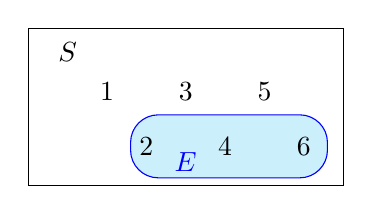
\begin{tikzpicture}
  \draw (-2, 2) rectangle (2, 0);
  \draw[rounded corners=10pt, fill = cyan!20, draw=blue] (-0.7,0.1) rectangle ++(2.5,0.8);
  \draw (-1.5, 1.7) node{$S$};
  \draw (-1, 1.2) node{1} (0, 1.2) node{3} (1, 1.2) node{5};
  \draw (-0.5, 0.5) node{2} (0.5, 0.5) node{4} (1.5, 0.5) node{6};
  \draw[text = blue] (0, 0.3) node{$E$};
\end{tikzpicture}
\caption{Sample space (the outcomes of a fair six-sided die) and event (rolling an even number) illustrated with Venn diagram}
\label{fig:probability-event}
\end{figure}

\emph{Probability} is a number between zero and one which tells us how likely an event to occur. If we assume (for now) that the sample space is finite and each possible outcome in an experiment  has an equal chance to occur, then the probability of event $E$ is
  \begin{equation}
    P(E) =\frac{\text{size of } E}{\text{size of } S}.
  \end{equation}
  In the example depicted in Figure~\ref{fig:probability-event} the probability that we roll an even number when we use a fair die, is $P(even)=3/6=0.5$.
  
In the following chapters we will deal with infinite (even uncountable) sample spaces, and we will generalize the definition of $P(E)$ then.
  
 \begin{example}[Elevator waiting time]
  Mr. Smith works on the 13th floor of a 15 floor building. The only elevator in his building  moves continuously through floors 1, 2, . . . 14, 15, 14, . . . 2, 1, 2,  . . . , except that it stops on a floor on which the button has been
  pressed. Assume that time spent loading and unloading passengers is very small
  compared to the traveling time.  Mr.~Smith complains that at 5pm, when he
  wants to go home, the elevator almost always goes up when it stops on his
  floor. What is the explanation?
\end{example}

When Mr.~Smith gets to the elevator, it may be below the 13th floor or above
it. The elevator will go up if it is below the 13th floor and it will go
down if it is above the 13th floor. There are 12 floors below the 13th floor and
2 floors above it, so the probability that the elevator is below the 13th floor
is $12/14\approx0.86>0.5$. Thus no matter when Mr. Smith wants to go home, it is
more likely that the elevator is going up.

We can simulate this situation:

\showCode{R}{Code/probability-elevator.R}
\runR{Code/probability-elevator.R}{elevator}{}
Running the above code should give:
\includeOutput{elevator}

  
\hypertarget{conditional}{%
\subsection{Conditional Probability}\label{conditional}}

When there are two events $A$ and $B$ under consideration, knowing that $A$ has occurred may change the probability for $B$ to occur. For example, suppose that someone rolls a die behind a curtain and tells us only that the number is less than or equal to 3. What is the probability that it is an even number? Given that we got 1, 2, or 3, the only possibility that it is even is if the number is 2. The \emph{unconditional} probability of getting an even number in a roll of a die is 1/2, but because of the information that provided to us, we conclude that the \emph{conditional} probability is 1/3. 
Using mathematical notation, we write  $P(B\mid A)=1/3$ which stands for ``conditional on $A$=the number is less than or equal to 3, the probability of $B$=the number is even, is 1/3''. 

Once again, it is helpful to visualize such things using a Venn diagram. In Figure~\ref{fig:probability-conditional}, the sample space $S$ consists of the six possible outcomes and the two events are depicted as a circle (event $A$) and as a rounded rectangle ($B$). To say that we condition on $A$ means that we restrict our view and look only at outcomes that could occur if we are told that $A$ has occurred. In other words, our sample space becomes $A$, instead of the whole set, $S$.

\begin{figure}[htbp]
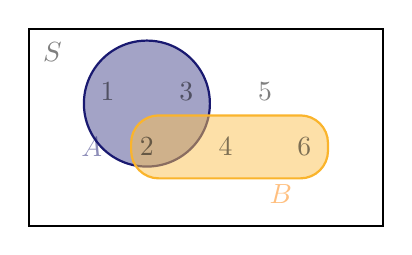
\begin{tikzpicture}[thick,fill opacity=0.5]
  \draw (-2, 2) rectangle (2.5, -0.5);
\draw[fill=MidnightBlue!80, draw=MidnightBlue] (-0.5, 1.05) circle (0.8);
  \draw[rounded corners=10pt, fill = Dandelion!80, draw=Dandelion] (-0.7,0.1) rectangle ++(2.5,0.8);
  \draw (-1.7, 1.7) node{$S$};
  \draw (-1, 1.2) node{1} (0, 1.2) node{3} (1, 1.2) node{5};
  \draw (-0.5, 0.5) node{2} (0.5, 0.5) node{4} (1.5, 0.5) node{6};
  \draw[text = orange] (1.2, -0.1) node{$B$};
  \draw[text = MidnightBlue] (-1.2, 0.5) node{$A$};
\end{tikzpicture}
\caption{Conditional probability -- given that we are told that a die gave a number less than or equal to 3 (event $A$), what is the probability that we got an even number ($B$)?}
\label{fig:probability-conditional}
\end{figure}

\bigskip
Can it be that we are told that some event $A$ has occurred, but this information tells us nothing about the probability of another event, $B$? Yes -- in this case we say that the two events are \emph{independent}, and we have
$$P(B\mid A) = P(B)\,.$$

For example, Abby rolls a fair die, while her roommate Amelia tosses a fair coin at the same time. If $A$ is the event `Abby got a 6' and $B$ is the event `Amelia got Heads', then $P(B\mid A) = 1/2$ because Abby's result has no impact on Amelia's. 

Sometimes establishing that two events are independent is harder. For example,
in general, the probability that Abby gets a text message within any given hour
is 0.7, and Amelia's is 0.6. Given that Abby got a text between 8 and 9am, does
it change the probability that Amelia got a text during the same hour? It may
depend on other (latent) events. For example, if they are late paying the rent,
then it is quite reasonable that Amelia will get a text from their landlord at
approximately the same time as Abby. 

Another related notion is that of `mutually exclusive' events. For example, suppose that
the Golden State Warriors and the Boston Celtics make it to the NBA finals. If
$A$ =  the Golden State Warriors will win the NBA championship next season, and
$B$ = the Boston Celtics will win the NBA championship next season, then these
events cannot occur at the same time. Mutually exclusive events are not independent. In
this example, if we somehow know that $A$ has happened, then we know for sure
that $B$ will not. Moreover, if we assign a probability of 0.6 that the Golden
State Warriors will win, then we know that $P(B) = 0.4$. 

\begin{example}[Two Children]
Consider the following two problems:
\begin{enumerate}
\item Mr. Jones has two children. The older child is a girl. What is the
  probability that both children are girls?
\item Mr. Smith has two children. At least one of them is a girl. What is the
  probability that both children are girls?
\end{enumerate}
\end{example}
In a family with two children there are four possible combinations of boy/girl
when we take into consideration their ages: \{Boy, Boy\}, \{Boy, Girl\}, \{Girl,
Boy\}, and \{Girl, Girl\}. Suppose that they all have the same probability to
occur.

For the first question: the sample space for the given situation consists of only two events -- \{Girl, Boy\}, \{Girl, Girl\}; and only one of them corresponds to the event of having two girls. Thus the
probability of two girls is 1/2. This question can also be solved this
way: since the older child is a girl, the probability of two girls is the
probability that the younger child is a girl which is 1/2.

For the second question, the sample space includes three possibilities: \{Boy, Girl\}, \{Girl, Boy\}, \{Girl, Girl\}. Thus the
probability of having two girls, given that at least one of them is a girl, is 1/3.

If we simulate many families, we can find the numerical answer quite accurately.

\showCode{R}{Code/probability-TwoChildren.R}
\runR{Code/probability-TwoChildren.R}{TwoChildren}{}
Running the above code should give:
\includeOutput{TwoChildren}





\subsection{Bayes' Rule}\label{Bayes}
One of the most important results in probability and statistics looks deceivingly simple, but has deep consequences, as we'll see in some of the subsequent examples. It is called Bayes' Rule, named after the reverend Thomas Bayes who discovered it in the 18th century. Consider two events, $A$ and $B$, such that $P(A)$ is greater than zero. Then
\begin{equation}\label{eq:bayes}
  P(B\mid A) = \frac{P(A\mid B)P(B)}{P(A)}.
\end{equation}
This formula is very useful when the conditional probability $P(B\mid A)$ is
difficult to find but the conditional probability $P(A\mid B)$ as well as the
unconditional probabilities are easy to find.

 \begin{example}[Football or ballet?]
Jane has season tickets to the home games of her town's football team, which she
attends 80\% of the time, and she also has season tickets to the town's ballet
which she attends 20\% of the time. If she attends the ballet in a week, she
will flip a fair coin to decide if she will attend the football game.
% In 10\% of the weeks she attends both the weekly football game and the ballet. 
This is depicted in Figure~\ref{fig:bayes-rule}, which shows that $P(F)=0.8$ and
$P(B)=0.2$. If we see Jane in the ballet, what is the probability that we'll see
her in the game in the same week?

% If we see her in the ballet, what is the probability that we will see her in the football game, as well?
% With Bayes' rule we get $P(A\mid B) =0.125\times0.8/0.2=0.5$.
% So, although Jane goes to  80\% of the football games, if she ends up going to the ballet then she is less likely to go to the game in the same week (50\%). 
\end{example}

We know that if we see her in a game, then the probability of seeing her in the
ballet is $P(B \mid F)=0.5$. Using Bayes' rule, $P(F\mid B)
=0.5\times0.2/0.8=0.125$.

\begin{figure}[H]
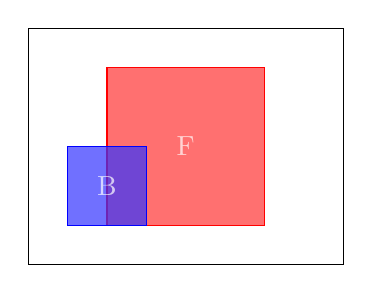
\begin{tikzpicture}[fill opacity=0.7]
  \draw (0,3) rectangle (4, 0);
  \draw[fill = red!80, draw=red] (1, 0.5) rectangle ++(2,2) node[midway,white]{F};
  \draw[fill = blue!80, draw=blue] (0.5,0.5) rectangle ++(1,1)  node[midway,white]{B};
\end{tikzpicture}
\caption{Bayes' rule. $F$ is the event that Jane attends the weekly football game, and $B$ is the events that she attends the weekly ballet}
\label{fig:bayes-rule}
\end{figure}



\begin{example}[Bertrand's Box]
Bertrand's box paradox was first posed by Joseph Bertrand in 1889. Here's the
question: there are three boxes, one contains two gold coins, one contains two
silver coins, and one contains a gold coin and a silver coin.
A box is selected at random and a coin is taken from that box at random. If the
coin is a gold coin, what's the probability that the other coin in that box is
also a gold coin?
\end{example}

This problem is about conditional probability. It's easy to find the
probability of getting a certain box, and it is easy to find the probability of
getting a gold coin if we know the box, as shown in
Figure~\ref{fig:probability-flow}. However, it is non-trivial to find the
probability of getting a certain box after we take out just one coin.
%when we know the final coin.
We see the six
possible outcomes in Figure~\ref{fig:probability-flow} are equally likely to
occur. Two outcomes of a gold coin are through the path of the box with two gold
coins and one outcome of a gold coin is through the path of the box with a gold
coin and a silver coin. Thus the answer to this problem is 2/3.

\begin{figure}[H]
\resizebox{0.6\columnwidth}{!}{%
\begin{tikzpicture}[%scale=0.5,
  edge from parent/.style={draw,-latex},
    boxes/.style={star, draw=none, fill=red, drop shadow, text centered, anchor=north},
    state/.style={draw=none, fill=red, circle, drop shadow, text centered, anchor=north},
    leaf/.style={draw=none, fill=orange, ellipse, text centered, anchor=north},
    leafs/.style={draw=none, fill=gray, ellipse, text centered, anchor=north},
    level distance=0.9cm, growth parent anchor=south
]
\node [boxes] {Boxes} [->] [sibling distance=4cm]
child{ [sibling distance=2cm]
  node [state] {Gold, Gold}
  child{node [leaf] {Gold}
    edge from parent{node[left]{$\frac{1}{2}$}}
  }
  child{node [leaf] {Gold}
    edge from parent{node[right]{$\frac{1}{2}$}}
  }
  edge from parent{node[above right]{$\frac{1}{3}$}}
}
child{ [sibling distance=2cm]
  node [state] {Gold, Silver}
  child{node [leaf] {Gold}
    edge from parent{node[left]{$\frac{1}{2}$}}
  }
  child{node [leafs] {Silver}
    edge from parent{node[right]{$\frac{1}{2}$}}
  }
  edge from parent [dashed] {node[right]{$\frac{1}{3}$}}
}
child{ [sibling distance=2cm]
  node [state] {Silver, Silver}
  child{node [leafs] {Silver}
    edge from parent{node[left]{$\frac{1}{2}$}}
  }
  child{node [leafs] {Silver}
    edge from parent{node[right]{$\frac{1}{2}$}}
  }
  edge from parent [dashed] {node[above right]{$\frac{1}{3}$}}
};
\end{tikzpicture}
}
\caption{Probability flow for Bertrand's Box}
\label{fig:probability-flow}
\end{figure}

This problem can also be solved using the Bayesian formula in
(\ref{eq:bayes}). Let $A$ be the event of getting a gold coin and $B$ be the
event of getting a box with two gold coins, then $P(A)=1/2$,
$P(B)=1/3$, and $P(A|B)=1$. Now the probability of a box with two gold
coins given a final gold coin is 
\begin{align}
  P(B\mid A) = \frac{P(A\mid B)P(B)}{P(A)}
  = \frac{1\times\frac{1}{3}}{\frac{1}{2}}
  =\frac{2}{3}.
\end{align}

Both of the aforementioned approaches give us the correct answer. However,
we don't have to go through the counting or reasoning. If we can simulate the
game, we can find the result pretty accurately. The following code simulates the 
game and approximate the probability numerically.

\showCode{R}{Code/probability-BertrandBox.R}
\runR{Code/probability-BertrandBox.R}{BertrandBox}{}
Running the above code should give:
\includeOutput{BertrandBox}

\section{When Intuition May Fail}
Probability-based logic may be confusing and even counter-intuitive in some cases. In this section, we show such cases, some of which have confused some of the brightest people. The purpose of introducing these examples is to show how they may occur in everyday situations, and how to deal with them correctly.

\hypertarget{Intransitive-Dice}{%
  \subsection{Intransitivity -- when $A>B$ and $B>C$ does not imply $A>C$}\label{Intransitive-Dice}}
Real numbers are transitive, meaning that if we know that $x>y$ and $y>z$ then $x>z$. However, probabilities of events are not always transitive. 
\begin{example}[Intransitive Dice]
We have three unusual dice:
\begin{itemize}
\item Die A has sides 2, 2, 4, 4, 9, 9.
\item Die B has sides 1, 1, 6, 6, 8, 8.
\item Die C has sides 3, 3, 5, 5, 7, 7.
\end{itemize}
\end{example}

To play a game you and your opponent choose two of the dice, say, A and B, and you get to choose which die you roll (and your opponent will roll the other.) The one who tolls a larger number wins. Which die do you want to choose?

Let's tabulate the possible results if dice A and B were chosen, and see which  die is preferred.
\begin{table}[H]
  \begin{tabular}{cc|ccc}
    \toprule
    &   & \multicolumn{3}{c}{B} \\
    &   & 1                & 6                & 8                \\
    \midrule
    \multirow{3}{*}{A}
    & 2 & \color{red}$A>B$ & $A<B$            & $A<B$            \\
    & 4 & \color{red}$A>B$ & $A<B$            & $A<B$            \\
    & 9 & \color{red}$A>B$ & \color{red}$A>B$ & \color{red}$A>B$ \\
    \bottomrule
  \end{tabular}
\end{table}
Since die A wins five out of the nine possible results and all possible results
occur with equal probability, we know that die A has a higher winning
probability (5/9) than die B. We should choose die A over die B.

Now suppose we choose dice B and C.
\begin{table}[H]
  \begin{tabular}{cc|ccc}
    \toprule
    &   & \multicolumn{3}{c}{B}                       \\
    &   & 1                & 6                & 8     \\
    \midrule
    \multirow{3}{*}{C}
    & 3 & \color{red}$C>B$ & $C<B$            & $C<B$ \\
    & 5 & \color{red}$C>B$ & $C<B$            & $C<B$ \\
    & 7 & \color{red}$C>B$ & \color{red}$C>B$ & $C<B$ \\
    \bottomrule
  \end{tabular}
\end{table}
We see that die B has a higher winning probability (5/9) than die C,
so we should choose die B over die C.

Since we should choose die A over die B, and choose die B over die C, does this
mean that we should choose die A over die C if these two dice are to be
selected? Surprisingly, the answer is NO. Here is the table of the possible
results.
\begin{table}[H]
  \begin{tabular}{cc|ccc}
    \toprule
    &   & \multicolumn{3}{c}{C} \\
    &   & 3                & 5                & 7                \\
    \midrule
    \multirow{3}{*}{A}
    & 2 & $A<C$            & $A<C$            & $A<C$            \\
    & 4 & \color{red}$A>C$ & $A<C$            & $A<C$            \\
    & 9 & \color{red}$A>C$ & \color{red}$A>C$ & \color{red}$A>C$ \\
    \bottomrule
  \end{tabular}
\end{table}
We should choose die C over die A!

Here is an experiment to simulate the intransitive dice.

\showCode{R}{Code/probability-IntransitiveDice.R}
Running this code should give the following:
\runR{Code/probability-IntransitiveDice.R}{IntransitiveDice}{}
\includeOutput{IntransitiveDice}


You are probably never going to encounter such dice, or play this game, but you may encounter a similar situation in real life when you have to choose among different people for a single position, or choose among similar products, based on preferences or ratings.
For example, suppose you want to purchase a new phone which is offered by three manufacturers, and there are six reviews for each phone. Note that the average ratings of all three options in our made-up example is the same. You may prefer phone A because it got the highest rating (twice). However, it also got two very low ratings, so choosing based on the maximum is risky. Option C has less variability in its ratings, but it didn't get a very high score from any reviewer. Furthermore, it may be that you have 60,000 reviews for each phone, and not just six. So, going systematically over the reviews is impractical, and you may decide that the best way to choose your phone is to use a randomized algorithm like the one in the dice example. That is, choose two of the options, and  then choose one random rating for each one, and select the one that give the highest score. This is a reasonable algorithm, but you have to be aware of the fact that when choices are made based on a probabilistic approach, ordering of options may not have the transitive property.



\hypertarget{birthday-problem}{%
  \subsection{Seemingly Rare Events}\label{birthday-problem}}

\begin{example}[Birthday Problem]\label{exam:birthday}
You go on a long trip on your birthday and take a bus. There are 23 people on
the bus, and to make the ride more fun you ask all the other passengers for
their birth date (month and day, not year) and see if you can celebrate
together. How likely is it that someone on the bus shares your birthday? How
likely are there at least two of the other 23 people who share a birthday (even
if it's not the same as yours)?
\end{example}

The chance that a random person has the same birthday as yours is
$1/365\approx0.0027$, so this is a rare event.
With 23 other people on the bus, the probability that someone shares your
birthday is about $0.061$ which is quite small, so it is pretty unlikely. For
the second question that two of the 23 people share a birthday, it seems that
the answer is similar, but the actually probability is surprisingly much
higher. The probability that at least two people share a birthday is about 0.5.

If you took a plane with 253 passengers, the probability that someone shares
your birthday is around 0.5. But you are almost certain that at least two people
share a birthday on that plane, because the probability is almost one.

% We will also answer the following question: what is the probability that on the bus/plane there are at least two people who share a birthday (even if it's not the same as yours)?

Let's use simulation to find answers to these questions.

\showCode{R}{Code/probability-birthday.R}
\runR{Code/probability-birthday.R}{birthday}{} Running the above code gives
results which are very close to the number we stated above, as predicted by
probability. That is, if there are 23 other people on the bus the probability
that some person's birthday is the same as yours is
\inlnR{```cat(prob.p23[1])```} and the probability that some other people share
the same birthday is \inlnR{```cat(prob.p23[2])```} . If there are 253 people on
the plane, the two probabilities are \inlnR{```cat(prob.p253[1])```} and
\inlnR{```cat(prob.p253[2])```}, respectively.

This example shows that some seemingly rare events are not rare, and they occur
quite often, especially when we get mutiple samples. %The second event has a large probability to occur, because the
%number of possible pairs is much larger.
When you want to see if any of the 23
people has the same birthday as yours, there are only 23 pairs to consider for the event to occur
(comparing your birth date with each of the birth dates of the other people). When you want to see if
any of the 23 people share the same birthday, there are $23\times22/2=253$ possible pairs
(each two persons of the 23) to consider for the event to occur.

This is particularly important in trials, where DNA match is often
used as evidence that a defendant has committed a crime. The chance that a DNA
sample from a particular crime scene matches a random person is extremely low,
but not zero. With nine billion people in the world and many crime scenes, the
probability that some other person's DNA (other than the true offender) matches
the DNA sample from a scene is not negligible.

\begin{listhead}\color{red}
\item [Exercise] Adapt the previous code by changing $N$ and $n$, to check the
  probability that someone will be selected multiple times if you pick a
  name from a list of one million names for one thousand times.
\end{listhead}

\subsection{Predictions}
The following example is one of the earliest questions in probability, when the field was mostly of interest among gamblers (who were also prominent mathematicians).

\begin{example}[Fair Division]
Tom and Jerry each put 30 dollars in a jackpot to start a tennis match. They are
equally good players, and have equal chance to win a match. They decide that the
first one to win three matches will win the \$60.  Now, Tom has won twice and
Jerry has won once, but the matches took a long time and they had to go back
home before a winner was declared. How should they split the 60 dollars, given
the current position (Tom leading 2-1)?
\end{example}

It seems Tom has won twice and Jerry has won once so the 60 dollars should be
split as $40:20$. However, this split is proportional to their current scor, but
it's not proportional to their probabilities of
winning. They need at most another two matches in order to know the final winner. Here are
the four possible winners of the next two matches: \{Tom, Tom\}, \{Tom, Jerry\},
\{Jerry, Tom\}, and \{Jerry, Jerry\}. In the first three possible outcome Tom
ends up with 3 wins, and therefore would get the \$60, and only the fourth
outcome leads to Jerry being the first to reach three wins.
So the probabilities that Tom and Jerry would be the final winner are 3/4 and
1/4, respectively, and thus the fair division should be $45:15$.

Let's use simulation to solve this problem.

\showCode{R}{Code/probability-FairDivision.R}
\runR{Code/probability-FairDivision.R}{FairDivision}{}
Running the above code should give:
\includeOutput{FairDivision}

The takeaway from this example is that it is not sufficient to know what has
happened in the past in order to make accurate predictions. It's also necessary
to know the `horizon' of the experiment (how much longer the experiment needs to
run.) The same logic would apply if the winning probabilities in each match are
not equal, and when the horizon is farther (more matches are needed in order to
declare the winner.)

This can be applied in financial disputes over inheritance. Suppose that Tom and
Jerry are heirs to a big fortune and the go to court, each one hoping to get the
full amount. It may be a lengthy procedure, and maybe at some point they feel
that Tom is leading in the eyes of the judge, but they know that the process may
continue for a long time and they might even die before a decision is made. So,
they can reach a settlement on their own, and avoid the remaining legal
proceedings. This is an oversimplified situation, because there is no clear
score as in a game, but the main idea is that the horizon is as important as the
past in making such decisions.

\hypertarget{Monty-Hall-problem}{%
\subsection{Jumping Probabilities}\label{Monty-Hall-problem}}

\begin{example}[Monty Hall Problem]
Suppose you're on a game show, and you're given the choice of three doors:
Behind one door is a car; behind the others, goats. Whichever door you pick, you
get what's behind it.  You pick a door, say No. 1, and the host, who knows
what's behind the doors, opens another door, say No. 3, which has a goat. He
then says to you, ``Do you want to pick door No. 2?'' Is it to your advantage to
switch your choice?
\end{example}

This famous example has confused many smart people. It's also about conditional
probability and can be solved by using the Bayesian formula. However, setting up
the conditional and unconditional probabilities for this problem is
complicated. Some people did not believe the result answer until they were shown some
simulations. The following code provide a simulation based on \code{n=1000}
repetitions.   

\showCode{R}{Code/probability-MontyHall.R}
\runR{Code/probability-MontyHall.R}{MontyHall}%[run]
Running the above code should give:
\includeOutput{MontyHall}

We see that the probability of winning a car is much higher than 0.5 if one
chooses to switch.

We initially have no information where the prize is, so the probability that the
prize is behind any door is 1/3. Intuition often fails in the second step: when
another door is opened and it contains no prize, most people think that the
total probability has to be divided equally between the two remaining doors. In
other words, the 1/3 probability that we assigned to door 3 has to be divided in
two, and 1/6 will go to the probability of each of doors 1 and 2
(1/3+1/6=1/2). But this is wrong!

Does the fact that we picked initially door 1 (completely by chance) makes any
of the doors special somehow? Strangely, yes!  When we pick door 1 there are two
possibilities -- either it's the winner (with probability 1/3) or it's not. If
it is, then the host can choose either door 2 or door 3 to open (each with
probability 1/2). However, if door 1 is not the winning door, then the host has
no choice. If door 2 is the winner then he must open door 3.  Since we know he
opened door 3, either door 1 is the winner and the host opened door 3 with
probability 1/2 or door 2 is the winner and the host opened door 3 with
probability 1. So, the probability that the host opened door 3 if door 2 is the
winner is twice the probability he opened door 3 if door 1 is the winner.

Notice that this not a consequence of the host trying to trick us, or we having
to perform some reverse psychology and trying to guess what the host
thinks. It's purely a consequence of conditioning on what has already happened
and the information it revealed about the possible future outcome.

\hypertarget{simpsons-paradox}{%
\subsection{Beware of generalizations}\label{simpsons-paradox}}
If we observe a delay in flight take-offs in 8 out of 10 airports, can it be
that overall in the country the average flight takes off on time? If the average
admission rate in a university is greater for women than for men, can it be that
in many (or even most) departments in that university the admission rate for men
is greater than for women? The answer to both these questions, and many similar
scenarios in life, is yes. This phenomenon is called Simpson's paradox.

\begin{example}[Combined percentages]
Tanya and Sonya are two freshmen players in college. In the first 3 games of the
season, Tanya had 11 free throws of which she made 6, and Sonya went 7 times and
made 4 of the free throws.  If at the end of game three the coach want to pick
the player with the best chance of making free throws, who should she choose?

Tanya's probability based on the first three games is $5/11 = .455$, while
Sonya's is $3/7 = .429$, so if the coach picks Tanya the team has a better
chance from the free throws line.

During the next three games, Tanya got 9 free throws and made 6, and Sonya got
14 free throws and made 9.  Again, at the end of game six the coach has to
choose the better free-throw shooter. Based on the last 3 games, Tanya's chances
are $6/9 = .667$, while Sonya's are $9/14 = .643$. So once again, the coach
picks the player with the better chances, and based on the last three games, it
is Tonya once again.

However, if we combine the results from all six games we see that Tanya went to
the line 11+9=20 times and made 11 of the free throws, and Sonya got 7+14=21
free throws and made 3+9=12. So, if we combine the results from all six games
Tonya's percentage from the free throw line is 55\%, while Sonya's is 57.1\%, so
based on the cumulative information Sonya should be the coach's pick!
\end{example}

\begin{example}[UC Berkeley alleged gender bias]
A famous example of Simpson's paradox is a study of gender bias among graduate
school admissions to University of California, Berkeley. In 1973 UC Berkeley was
sued for sex-discrimination. Here are the overall numbers \textit{combined} from
the six largest departments in fall admission of 1973.

\begin{table}[H]
  \begin{tabular*}{\textwidth}{@{\extracolsep{\fill}}crrcrr}
    \toprule
    \multicolumn{3}{c}{Men} & \multicolumn{3}{c}{Women} \\
    \cmidrule(lr){1-3}\cmidrule(lr){4-6}
    Applicants & \multicolumn{2}{c}{Admitted} & Applicants
                                              & \multicolumn{2}{c}{Admitted} \\
    \midrule
    2691 & 1198 & ({\bf 44.5}\%) & 1835 & 557 & (30.4\%) \\
    \bottomrule
  \end{tabular*}
\end{table}

This table shows that men were much more likely than women to be admitted (by
14.1\%). Was there a gender bias? Let's break it down by department (which we
call A--F):

\begin{table}[H]
\begin{tabular*}{\textwidth}{@{\extracolsep{\fill}} ccrrcrr}
  \toprule
  & \multicolumn{3}{c}{Men}  & \multicolumn{3}{c}{Women} \\
  \cmidrule(lr){2-4}\cmidrule(lr){5-7}
  Department & Applicants  & \multicolumn{2}{c}{Admitted} & Applicants
                           & \multicolumn{2}{c}{Admitted} \\
  \midrule
A & 825 & 512& (62\%) & 108 & 89 &(\textbf{82\%})  \\ 
B & 560 & 353& (63\%) & 25  & 17 &(\textbf{68\%})  \\
C & 325 & 120& (37\%) & 593 & 202& (34\%) \\
D & 417 & 138& (33\%) & 375 & 131& (\textbf{35\%}) \\
E & 191 & 53 & (28\%) & 393 & 94 &(24\%)  \\
F & 373 & 22 & (6\%) & 341 & 24 &(\textbf{7\%})  \\
  \bottomrule
\end{tabular*}
\end{table}

Things get strange after we divide the data according different departments. In
four of the departments (A, B, D, and F) women were more likely to be admitted
than men.  In departments C and E, men were more likely to be admitted (by
3-4\%). In contrast, the acceptance rate for women in department A was 20\% more
than for men.

To explain this, \cite{bickel1975sex} noticed that women
tended to \textit{apply} to more competitive departments (C and E) with low admission
rates even among qualified applicants, whereas men tended to apply to
less competitive departments with high admission rates among the
qualified applicants.

So, this is not a case of gender discrimination, but rather, what's called
`confounding bias'. If women were more likely to apply to a competitive
department than men, the overall rejection rate among women can be expected to
be higher.  Consider an extreme example, with department X accepting 1\% of the
applicants, and department Y accepting 50\%. Suppose that 500 women choose to
apply to department X and 500 other women apply to department Y, and suppose
that 1000 men all apply to department Y. Then, department X will have 5 students
(all women) and will reject 495 of the applicants (again, all women). Department
Y, on the other hand will accept 500 men and 250 women. Overall, the acceptance
rate for women is $(5+250)/1000=0.255$, while for men it is $500/1000=0.5$.
\end{example}

Simpson's paradox is not limited to the scenarios of combined percentages or
confounding bias. To illustrate it, we use the following example via
simulations.

\begin{example}[Reverse trends]
We use the following code to simulate data from four groups, each with 40
samples.

\showCode{R}{Code/probability-Simpson.R}[1][6]
\runR{Code/probability-Simpson.R}{Simpson}{}
% Running the above code gives:
% \includeOutput{Simpson}

Next, we plot the whole data and fit a trend equation. Clearly, we see in the
left panels of Figure~\ref{fig:probability-simpson} that as $x$ increases $y$
increases.

\showCode{R}{Code/probability-Simpson.R}[8][9]

If we mark the points by the group to which they belong, and fit a trend line
separately for each group, as $x$ increases $y$ decreases in each and every
group!
\showCode{R}{Code/probability-Simpson.R}[10][12]


\begin{figure}[H]
\includegraphics[width=0.45\textwidth]{images/chapter_3/probability-Simpson-plots.pdf}
\includegraphics[width=0.45\textwidth,page=2]{images/chapter_3/probability-Simpson-plots.pdf}
\caption{Scatter plot of the whole data without (left) and with (right) group labeled}
\label{fig:probability-simpson}
\end{figure}

\end{example}

The three examples all show that we should be very careful when analyzing data
and remember that proportions or trends which are observed in the entire
population may be very different when we break down the data into groups.


\hypertarget{further}{%
\section{Further Examples}\label{further}}

\begin{example}[Henry's Choice\footnote{\url{https://www.braingle.com/brainteasers/20227/loaded-revolver.html}}]
Henry has been caught stealing cattle, and is brought into town for justice. The
judge is his ex-wife Gretchen, who wants to show him some sympathy, but the law
clearly calls for two shots to be taken at Henry from close range. To make
things a little better for Henry, Gretchen tells him she will place two bullets
into a six-chambered revolver in successive order. She will spin the chamber,
close it, and take one shot. If Henry is still alive, she will then either take
another shot, or spin the chamber again before shooting.

Henry is a bit incredulous that his own ex-wife would carry out the punishment,
and a bit sad that she was always such a rule follower. He steels himself as
Gretchen loads the chambers, spins the revolver, and pulls the trigger. Whew! It
was blank. Then Gretchen asks, ``Do you want me to pull the trigger again, or
should I spin the chamber a second time before pulling the trigger?'' What
should Henry choose?
\end{example}

We know that the first chamber Gretchen fired was one of the four empty
chambers. Since the bullets were placed in consecutive order, one of the empty
chambers is followed by a bullet, and the other three empty chambers are
followed by another empty chamber. So if Henry has Gretchen pull the trigger
again, the probability that a bullet will be fired is 1/4.

If Gretchen spins the chamber again, the probability that she shoots Henry would
be 2/6, or 1/3, since there are two possible bullets that would be in firing
position out of the six possible chambers that would be in position.

Let's solve this problem using the following simulation.

\showCode{R}{Code/probability-HenryChoice.R}
\runR{Code/probability-HenryChoice.R}{HenryChoice}{}
Running the above code should give:
\includeOutput{HenryChoice}

% % \hypertarget{prisoners-problem}{%
% \subsection{100 Prisoners Problem}\label{prisoners-problem}%}

The technique of simulation is useful in finding answers in very complicated
problems. Consider the following example modified from
\cite{flajolet2009analytic}.

\begin{example}[100 Prisoners]
In a prison, there are 100 death row prisoners who are numbered from 1
to 100, and there is a room with 100 drawers labeled from 1 to
100. The director randomly puts one prisoner's number in each closed
drawer and offers a last chance. The prisoners enter the room, one
after another. Each prisoner may open and look into 50 drawers in any
order. The drawers are closed again afterwards. If, during this
search, every prisoner finds his number in one of the drawers, all
prisoners are pardoned. If some prisoner does not find his number, all
prisoners die. Before the first prisoner enters the room, the
prisoners may discuss strategy, but they cannot communicate once the
first prisoner enters the room.
\end{example}

The situation is hopeless if every prisoner selects fifty drawers at
random. The probability that a single prisoner finds his number is
0.5, so the probability that all prisoners find their numbers is
$0.5^{100} = 7.89\times10^{-31}\approx0$. However, a better strategy
is given in \citep{stanley2013algebraic}, which is described below:
\begin{enumerate}
\item Each prisoner first opens the drawer with his own number.
\item If this drawer contains his number he is done and was
  successful.
\item Otherwise, the drawer contains the number of another prisoner
  and he next opens the drawer with this number.
\item The prisoner repeats steps 2 and 3 until he finds his own number
  or has opened 50 drawers.
\end{enumerate}

This strategy is better than randomly opening because it utilizes the
information from other prisoners. For example, different prisoners all start
from opening different drawers, while it is almost certain that some prisoners
start from opening the same drawer if they start with a draw at random.

\begin{listhead}
\item [Exercise] Use simulation to find the probability that some prisoners
start from opening the same drawer if they all start with a draw at random.\\
\emph{Hint:} Consider the birthday problem in Example~\ref{exam:birthday}.
\end{listhead}

The probability of survival with the better strategy is complicated to derive
analytically.  In the following, we define two functions to simulate the method
of randomly openning 50 drawers and the better strategy, respectively.

\showCode{R}{Code/probability-100prisoners.R}[1][41]
\runR{Code/probability-100prisoners.R}{100prisoners}
\noindent If we run the following code
\showCode{R}{Code/probability-100prisoners.R}[43][46]
\noindent we should get the following two probabilities for randomly and smartly open the
drawers, respectively:
\includeOutput{100prisoners}

We see that opening drawers randomly has a survival probability of almost zero
while the smart strategy gives a survival probability close to 0.3.

% Axioms?
% inequalities
% football code

\section{Summary}
This chapter covered basic concepts of probability and provided examples on how
probability can help interpret real-life phenomena. Faced with counter-intuitive
and challenging probability problems, we were able to leverage numerical
simulation techniques to gain deeper insights and find solutions easily. Moving
forward, the next chapter will focus on two important probability theorems.

%%% Local Variables:
%%% mode: latex
%%% TeX-command-extra-options: "-shell-escape"
%%% TeX-engine: xetex
%%% TeX-master: "../sidsmain.tex"
%%% End:

%\runR{Code/llnclt_IQ.R}{llnclt_IQ}
\runR{Code/llnclt_roulette.R}{roulette}
\runR{Code/llnclt_texts.R}{texts}
\runR{Code/llnclt_Cauchy.R}{texts}
\runR{Code/llnclt_CLTexp.R}{cltsimexp}
\runR{Code/llnclt_CLTbinom.R}{cltsimbinom}
\runR{Code/llnclt_boygirl.R}{boygirl}
\runR{Code/llnclt_IQ2.R}{cltiq2}

\hypertarget{ch:llnclt}{%
%  \chapter{The Law of Large Numbers and the Central Limit Theorem}\label{ch:llnclt}}
\chapter{Laws of Large Samples: Where Chaos Becomes Order}\label{ch:llnclt}}
Benjamin Franklin once said `In this world nothing can be said to be certain,
except death and taxes'. Still, for all the uncertain things in life, and
especially in science where most theories cannot be proven correct, we would
like to be able to say something about how confident we are about a conclusion
we draw. To do that, scientists conduct an experiment in which they collect
data and check if it provides evidence in favor or against a proposed theory.
This chapter describes two of the most important results in probability and
statistics --- the law of large numbers and the central limit theorem. These
theorems explain why statistics works and is useful in so many situations! They
tell us that, if we collect enough data (and conduct a sensible experiment)
we'll be able to say to what extent we can trust our results, and also tell us
how much data we need in order to draw conclusions with a certain degree of
confidence. Without these results, conducting experiments would be meaningless,
no matter how many samples are collected.

\section{Introduction}
Let's start with a few simple examples which will be used in this chapter:
\begin{enumerate}
\item We get a random sample of 200 people and give them an IQ test. What is
the distribution of the scores in this sample? How close is it to the true
distribution of the whole population?\\ How likely is it that we find a person
with IQ greater than 150?\\
In order to be accepted to the Mensa club a person has to be in the top 2\% of
the IQ distribution. What is the minimum score required in order to be a Mensa
member?  \item The pockets of the roulette wheel are numbered from 0 to 36. In
number ranges from 1 to 10 and 19 to 28, odd numbers are red and even are
black. In ranges from 11 to 18 and 29 to 36, odd numbers are black and even are
red. There is a green pocket numbered 0 (zero). Suppose you want to bet on a
color, say, red, and if the ball lands in a red pocket your payoff is twice
your bet, and otherwise you lose your bet. What is the probability you win?
What is your expected payoff? Suppose you have \$10,000, and you bet one dollar
each time. How much money will you win or lose?.
\item Suppose that you get a text message every 6 minutes (a rate of 10 per
hour), and suppose that they arrive independently of one another, according to
some presumed distribution. How many messages do you expect to get on an
average day, between 8am and 8pm? 
%\item \hb{homework question?}As of June 16, 2021 Tony Snell from the Atlanta
%Hawks leads the NBA in 3pt accuracy with 53.8\%.
%If he takes 3pt 10 shots per game over the next 10 games, how many three-point shots do you expect him to make?
\end{enumerate}

The main paradigm in statistical inference and prediction in order to answer
such questions is to take a sample from the population we're interested in, and
choose a mathematical model which we believe represents the whole population.
Then we check if our model appears to be reasonable, in the sense that it fits the
data well. If it does, we can use the mathematical properties of the model to
draw conclusions about the population. By representing the sample using a
mathematical (probabilistic) formula, we essentially augment a finite sample to
an infinite one. Working with a formula/model for the data allows us to use the
`heavy artillery' of math, like finding maximum/minimum, computing areas under
the curve of the function, and so on. 

This chapter deals with inference which can be derived from the mean of a
population, and we show the (arguably) two most important results in statistics
-- the \emph{law of large numbers} (\emph{LLN}) and the \emph{central limit
theorem} (\emph{CLT}). Together, these two very general theorems make it
possible to draw conclusions about the whole population, from a single sample!
(as long as the sample represents the whole population and the sample
size is large enough).


\section{The Law of Large Numbers\index{Law of Large Numbers}}

\subsection{Example \#1 -- the IQ score}
%We get a random sample of 200 people and give them an IQ test. From this sample, we want to infer the true distribution in the entire population.

Suppose that the IQ in the general population has a normal distribution with
mean of 100 and  standard deviation of 15, and from this population we draw 200
people and calculate the sample mean and standard deviation, like so:

\showCode{R}{Code/llnclt_IQ.R}[1][4]
%\runR{Code/llnclt_IQ.R}{llnclt_IQ}

Run this code. You should get that the sample mean is
\inlnR{```cat(mean(samp1))```}[llnmsamp1] and the standard deviation is
\inlnR{```cat(sd(samp1))```}[llnssamp1]. Both are very close to the true values.

Let's pretend that just like in real life, we don't know the true distribution.
We propose a certain distribution and check if it fits. In the current
example, which we called \lstinline{samp1}, we want to check if the normal
distribution is a good model for our data.

\jy{QQ plot seems distracting here}
One way to check if a distribution fits our data is with a graphical tool
called the \emph{Q-Q plot}. A Q-Q plot is based on the simple (and very
important) idea that a distribution is determined by its \emph{quantiles}
(percentiles), 
so if the quantiles of our sample match the quantiles of the assumed
distribution, then the assumption is reasonable. Recall that we defined the
quantiles in Chapter~\ref{introdistributions}, so that the $q$-th quantile is a
number $x_q$, such that $q\times 100\%$ of the data are less than or equal to
$x_q$.  In our example the data has  \inlnR{```cat(n)```}[llnsampsize] data points, so we
can get \inlnR{```cat(n)```}[llnsampsize2] quantiles from our sample. If we draw the same
number of random numbers from the correct distribution, then their quantiles
will match the quantiles we got from our data (they will only match
approximately, because when we draw finite, random samples, there is always
some `noise'.)

When it's assumed that the data come from a normal distribution, we can use the
\lstinline{qqnorm()} function to check if the assumption is reasonable:
\showCode{R}{Code/llnclt_IQ.R}[7][8]

The points in the Q-Q plot in Figure~\ref{qqplot1} show the actual quantiles
(from the data, \lstinline{samp1}) versus the theoretical quantiles (those that
would be obtained if we drew a sample from a normal distribution). The points in
the graph lie very close to a straight line, indicating that the sample was
likely drawn from a normal distribution. (This is not surprising here because we
generated the sample this way. However, when we get a random sample and do not
know the true distribution, this plot is useful for checking whether our
mathematical model is reasonable.)

\begin{figure}[H]
\includegraphics[width=0.6\textwidth]{images/chapter_4/qqplot1.pdf}
\caption{A Q-Q plot}
\label{qqplot1}
\end{figure}



To understand what the Law of Large Numbers says, let's repeat the previous
simulation but vary the sample size ($n$) and see what happens to the
\emph{sample mean} as we increase $n$.

\showCode{R}{Code/llnclt_IQ.R}[12][22]

\jy{how about putting sample size on log scale:
   \lstinline{ns <- rep(10 * 2^(0:11), each = 10)}'}

In \wingding{1} we create a vector of sample sizes. We will generate a random
sample for each of these \lstinline{ns}. In \wingding{2} we initialize a vector
which will hold all the sample means (at first, they are set to zero). The
\lstinline{for} loop in \wingding{3} is the same as the previous demonstration,
but in each iteration we increase the sample size, which is the first argument
of the function \lstinline{rnorm()}. The mean from the $i$-th sample is stored
in the $i$-th position of the vector \lstinline{allMeans} (in \wingding{4}.)

Figure~\ref{LLNdemo} shows the results. We can see that as $n$ increases, the
sample mean gets closer to the true mean (100, in our simulation), which is
shown as a horizontal line.

\begin{figure}[H]
\includegraphics[width=0.5\textwidth]{images/chapter_4/LLNIQ.pdf}
\caption{Visualizing the Law of Large Numbers -- normal data}
\label{LLNdemo}
\end{figure}

We also see in Figure~\ref{LLNdemo} that the dispersion of the sample means
gets smaller as the sample size gets larger, but this is the result of the
\emph{Central Limit Theorem}, which will be discussed later in this chapter.

\subsection{Example \#2 -- the Roulette Wheel}
Here, the outcome is binary -- we either win or lose a bet. The probability of
winning if we choose the red color, is $18/37$.  Let's simulate 40 bets at the
roulette wheel, where, in each we put a dollar on red. Each bet is won with a
Bernoulli distribution, $Ber(18/37)$ and we repeat it 40 times. Equivalently,
we can look at it as a single binomial sample, with $n=40$ and $p=18/37$.

%\runR{Code/llnclt_roulette.R}{roulette}
\showCode{R}{Code/llnclt_roulette.R}[1][4]

Run this code. You should get in this particular sample of 40 bets, that the
probability of winning (the mean of \lstinline{samp2}) is
\inlnR{```cat(mean(samp2))```}[llnsamp2m] (greater than 0.5.) This seems great -- if we
keep going we might get rich! However, let's see what happens to the sample
mean (which is the probability of winning) as we increase $n$. The following
code is nearly identical to the one used in the previous example, except that
in this case we draw the random samples from a \emph{binomial} distribution (in
\wingding{1}.)

\showCode{R}{Code/llnclt_roulette.R}[7][17]

We see the results in Figure~\ref{LLNdemoBinomial}. As before, the sample mean
gets closer to the true mean of the distribution, $p=18/37$, which is
less than 0.5, so if we keep placing bets we will end up losing money. In fact,
we can check how much we will lose if we bet \$1 each time, and do it 10,000
times.

\begin{figure}[H]
\includegraphics[width=0.5\textwidth]{images/chapter_4/LLNroulette.pdf}
\caption{Visualizing the Law of Large Numbers -- binomial data}
\label{LLNdemoBinomial}
\end{figure}

To simulate what will happen if we play the roulette table 10,000 times, each
time putting a dollar on red, run the following code:

\showCode{R}{Code/llnclt_roulette.R}[20][24]

The probability of winning in this simulation should be
\inlnR{```cat(mean(roulette))```}[llnmeanroulette]. We bet on \$10,000 and we won
\inlnR{```cat(sum(roulette))```}[llnsumroulette] times, so our winnings amounted to
\inlnR{```cat(prettyNum(2*sum(roulette), big.mark = ","))```}[llnprettysum] dollars, which
means that we lost  \inlnR{```cat(prettyNum(10000-2*sum(roulette), big.mark = ","))```}[llnprettysum2] dollars.

To the casino it doesn't matter if one person bets \$1,000,000 or if 1,000
people each bets on \$1,000 -- in both cases the casino will win with
probability 19/37 and will have a positive net gain (you can't beat the house).
Casinos know that, and use the law of large numbers in order to ensure that in
the long run, they will win.


\subsection{Example \#3 -- Receiving Text Messages}
Let's simulate $n$ days, and in each one count the number of messages, assuming
they arrive independently from a Poisson distribution with rate=10. To do that,
run the following code:

%\runR{Code/llnclt_texts.R}{texts}
\showCode{R}{Code/llnclt_texts.R}[2][10]

In each day we count messages over 12 hours, so in \wingding{1} we multiply the
(hourly) random sample from the Poisson distribution by 12. Figure
\ref{LLNdemoPoisson} shows the results.

\begin{figure}[H]
\includegraphics[width=0.5\textwidth]{images/chapter_4/LLNtexts.pdf}
\caption{Visualizing the Law of Large Numbers -- Poisson data}
\label{LLNdemoPoisson}
\end{figure}

If we continue to get text messages at this fixed rate over a long period of
time, and we calculate the average daily messages (from 8am to 8pm) we see that
that average converges to 12*10=120 messages per day.



\subsection{The LLN\index{LLN} -- an Intuitive Statement of the Theorem}
Informally, the law of large numbers states that the results of an experiment
tend to settle down to a fixed average when the experiment is repeated many
times. In other words, as the sample size increases, the sample mean will get
closer to the true population mean.

The LLN is very general -- it doesn't matter if the question is about how many
boy-births we expect to see (\emph{binomial distribution}), the number of
received text messages (\emph{Poisson distibution}), or if we measure IQ
(\emph{normal distribution}). The only requirements are that the samples are
independent, and identically distributed, and that the true distribution
actually has a mean. (We will see an example where this is not the case.)

It's important to emphasize that the LLN doesn't imply that the results of
future experiments will balance out what already happened! If we bet 100 times
at the roulette wheel and lost each time, this doesn't mean that we have a
better chance of winning the next bet. All the LLN is saying is that if we
continue to play many times, the overall probability that we win in each round
will converge to 18/37.

\subsection{Example \#4 -- When the LLN\index{LLN} Doesn't Work}
We have two groups of students who have to take a math test. Group A has a mean
score of 70 and a standard deviation of 10, while group B has mean 60 and
standard deviation 20. Both groups have a normal distribution.  We take a
sample of size $n$ from each group and calculate the sample means. Then, we
calculate the difference between the sample means,
$d_{AB}=\bar{x}_A-\bar{x}_B$, and the ratio between the means,
$r_{AB}=\bar{x}_A/\bar{x}_B$.
As before, we increase the sample size and see how it affects $d_{AB}$ and $r_{AB}$.

%\runR{Code/llnclt_Cauchy.R}{texts}
\showCode{R}{Code/llnclt_Cauchy.R}[2][19]

In \wingding{1} and \wingding{2} we generate the samples from the two groups
(both follow a normal distribution), with the same sample size. In the \lstinline{for} loop
we vary the sample size to go from 50 to 5,000 in jumps of 10. In \wingding{3}
and \wingding{4} we calculate the difference and the ratio between the mean
scores in the two groups, respectively. In \wingding{5} and \wingding{6} we
keep the calculated values $d_{AB}$ and $r_{AB}$ in vectors called
\lstinline{allDiffs} and \lstinline{allRatios}, which are then used in the
\lstinline{plot()} function.


Figure~\ref{LLNdemoCauchy}, which is what you should get after running the
code,  shows the distributions of the difference between the average grades
($d_{AB}$) on the left, and of the ratio ($r_{AB}$) on the right.  What we see
here is that the mean difference between the groups, $d_{AB}$, converges to the
true difference between the groups (10), but the ratio, $r_{AB}$, doesn't
converge -- $n$ can be as large as we want, and we will still see ratios that
are quite extreme. (Note that the mean of a ratio between two distributions is
generally not equal to the ratio of the means of the distributions, so we don't
expect $r_{AB}$ to converge to exactly 70/60.)

\begin{figure}[H]
\includegraphics[width=1\textwidth]{images/chapter_4/LLNCauchy.pdf}
\caption{When the Law of Large Numbers\index{Law of Large Numbers} fails}
\label{LLNdemoCauchy}
\end{figure}

\jy{If the normals do not have mean zero, the ratio is not exactly
  Cauchy but Cauchy like in tails.}
What is happening here? The answer is that while a difference between two
normal random variables is still normal (and therefore, has a mean), the ratio
between two normal distributions follows a \emph{Cauchy distribution} which
doesn't have a theoretical mean, so the LLN doesn't apply to the ratios
between the grades of the two groups,  $r_{AB}$.

Although the LLN applies to almost any distribution we will ever encounter, the
lesson here is that taking the ratio between two perfectly well-behaved
distributions may lead to a distribution to which the LLN doesn't apply. Other
manipulations of random variables may lead to similar results.



\section{The Central Limit Theorem\index{Central Limit Theorem}}
The LLN says that as we increase the sample size, the sample mean converges to
a fixed value (the true population mean).  It doesn't say anything, however,
about how close the sample estimate is to the true value. In other words, it
says nothing about our level of (un)certainty. 

The central limit theorem (CLT\index{CLT}) says that, in most situations, if we could get
many random samples from the population, and calculate the mean from each
sample, and then plotted the many sample means as a histogram, then this
histogram will look like a normal distribution. This is true even if the
original variables themselves are not normally distributed!

The CLT requires very little about the actual distribution of the data: the
sample has to be independent and identically distributed (i.i.d.), and the
distribution must have a finite variance. 
\jy{We only defined sample variance but not population variance so far.}

\subsection{CLT -- Examples}
We will draw a random sample of size $n$ from the following distributions:
\begin{itemize}
%\item Standard normal (the \lstinline{rnorm(n,0,1)} function).
%\item Poisson with rate parameter $\lambda=3$ (use \lstinline{rpois(, 3)}).
\item Exponential with rate parameter 5.5 (using \lstinline{rexp(n, 5.5)}).
\item Binomial with probability 0.15.
\end{itemize}

In each case, we will plot a histogram of the sample, and overlay the
probability density function on top of it.  We will repeat it 10,000 times and
each time calculate the sample mean. Then, we will plot a histogram of the
10,000 sample means.

\subsubsection{Exponential Distribution}
First, let's draw one sample from Exp(5.5) with $n$=100 random i.i.d. draws,
and see that the distribution of the sample is very different from normal. In
the following code, we plot a histogram from one sample (with n=100) and
overlay the graph of the probability distribution function of Exp(5.5), in
order to show that the sample is representative of the true distribution:

\showCode{R}{Code/llnclt_CLTexp.R}[2][7]
%\runR{Code/llnclt_CLTexp.R}{cltsimexp}

Notice that the distribution in Figure~\ref{CLTexp} is very skewed, and doesn't
look at all like a normal distribution. Try running \lstinline{mean(expsamp1)}. you
should get \inlnR{```cat(mean(expsamp1))```}[llnmeansampexp], which is approximately
1/5.5, the theoretical mean of the Exp(5.5) distribution.

\jy{Add sample size and exponential paraemters to caption.}
\begin{figure}[H]
\includegraphics[width=0.6\textwidth]{images/chapter_4/CLTexp.pdf}
\caption{Simulated data from an exponential distribution}
\label{CLTexp}
\end{figure}

To understand the CLT, we will draw 10,000 samples, calculate the mean of each
sample, and plot a histogram of those 10,000 sample means. We will first do it
with $n$=50, like so:

\showCode{R}{Code/llnclt_CLTexp.R}[12][22]

In \wingding{1} we prepare a vector which will hold the sample mean from 10,000
simulated datasets. In \wingding{2} we get the sample mean for the $i$th random
sample, and update the vector \lstinline{allMeans}. Then, we plot the histogram
and use \lstinline{abline} to show the true mean of the population (which is
1/5.5).

Repeat the same code, but change the first line to \lstinline{n <- 500}. Figure
\ref{CLTexp2} shows the results for $n=50$ (left) and $n=500$ (right).

\begin{figure}[H]
\includegraphics[width=0.9\textwidth]{images/chapter_4/CLTexp2.pdf}
\caption{The distribution of the sample mean from 10,000 simulated data from an
exponential distribution. Left: $n=50$, right: $n=500$} \label{CLTexp2}
\end{figure}

We can see that the mean is estimated quite accurately in both cases, and the
overall shape of the 10,000 sample means has the shape of a normal
distribution. However, the spread (variance) of the distribution decreases as
the sample size increases. This is the essence of the CLT!  It tells us that
the \emph{single} sample mean that we actually have is most likely not exactly
the true mean in the population, but if we can get a larger sample size ($n$)
then we'll know that the range in which we can expect to find the true mean is
getting smaller.

\subsubsection{Binomial Distribution}
In order to see the generality of the CLT, we demonstrate it again with
another, very different distribution. This time our data come from a discrete
and skewed distribution (the binomial).

The following code is very similar to the previous one, except that we use
\lstinline{rbinom} to generate the data. Try it, and then change the first line
to \lstinline{n <- 500}, and run it again.

\showCode{R}{Code/llnclt_CLTbinom.R}[3][13]
%\runR{Code/llnclt_CLTbinom.R}{cltsimbinom}

You should get the plot in Figure~\ref{CLTbinom}. Notice that because we've
simulated data with a relatively small probability of getting a success
($p$=0.15), when $n$=50 the shape of the distribution of sample means is still
a bit skewed, but when $n$ is large the bell shape appears!

\begin{figure}[H]
\includegraphics[width=0.9\textwidth]{images/chapter_4/CLTbinom.pdf}
\caption{The distribution of the sample mean from 10,000 simulated data from a
binomial distribution. Left: $n=50$, right: $n=500$} \label{CLTbinom}
\end{figure}

Once again, in both cases the mean of 10,000 simulated sample means is very
close to the true value (0.15), but as $n$ gets larger, we are more confident
that the \emph{only} value that we got from \emph{a single} experiment is close
to the true value, because the range in which we can find the true value is
narrower.

\subsubsection{Application to Child Births -- Boy/Girl Ratio}
In 2021 the boy to girl birth ratio in the USA is estimated to be 1.05. If we
took a random sample of 300 newborns across the USA, how many do you expect to
be boys? Run the following code:

\showCode{R}{Code/llnclt_boygirl.R}[1][8]
%\runR{Code/llnclt_boygirl.R}{boygirl}

This should give the following:
\includeOutput{boygirl}%[inline]

Would it be very surprising if we actually saw 148 in the random sample?
Suppose we took a sample of 3,000, instead. Would is be surprising if we
observed 1,480 boys?  How about if we took a sample of 30,000, instead. Would
is be surprising if we observed 14,800 boys?

The probability of a boy birth doesn't depend on the sample size, and we
calculated it to be 0.512, so the expected number of boys when the sample size
is 300, 3,000, and 30,000 is 151, 1,510, and 15,100, respectively. So, it may
appear that actually observing 148 instead of 151 is as likely as observing
1,480 instead of 1,510, or 14,800 instead of 15,100, but that is not true!  The
CLT tells us that when the sample size increases, the dispersion of the sample
means around the true mean gets smaller and smaller. This is demonstrated in
the code below. 
\showCode{R}{Code/llnclt_boygirl.R}[14][32]

The result is shown in Figure~\ref{CLTboygirl}.
The green vertical line represents the expected number of boys, and the red one
represents the observed ones. Notice that as we increase the sample size, the
likelihood of the observed number of boys (148, 1,480, 14,800) gets smaller.
When $n=30,000$ the red line is well outside the range of the simulated sample
means.

\begin{figure}[H]
\includegraphics[width=\textwidth]{images/chapter_4/CLTboygirl.pdf}
\caption{Number of boy births with different sample sizes ($n$=300, 3,000, and
30,000)} \label{CLTboygirl}
\end{figure}


\section{Application -- the  IQ Scores}
Let's revisit the IQ example, where we assumed that in the general population
IQ scores have a normal distribution with mean of 100 and  standard deviation
of 15.  We drew a sample of 200 people, and calculated the sample mean and
standard deviation, which turned out to be 99.4, and 15.6, respectively.

In the following code, we plot two curves on top of the histogram we obtain
from the sample -- one for the true normal distribution, and one using the
sample mean and sample standard deviation:
\showCode{R}{Code/llnclt_IQ2.R}[2][8]
%\runR{Code/llnclt_IQ2.R}{cltiq2}

Figure~\ref{CLTIQfit} shows the result. The red curve shows the true density
function, and the dashed green one shows the one estimated from the sample of
200 people. They are very close. The LLN tells us that as we increase our
sample size, the sample mean will be closer to the true mean.  The CLT tells us
how close to the true mean we can expect that our sample mean to be. As the
sample size gets larger, our confidence in how close we are to the true value
increases (because the range of the values we can get from random sampling
becomes narrower.)

\begin{figure}[H]
\includegraphics[width=0.6\textwidth]{images/chapter_4/IQfit.pdf}
\caption{Distribution of 200 IQ scores}
\label{CLTIQfit}
\end{figure}


In order to answer the question how likely  it is to find a person with IQ
greater than 150, we can calculate the area of the right tail of the
distribution. We can do it with the following code:
\showCode{R}{Code/llnclt_IQ2.R}[11][11]
Try it. You should get that the probability to get a score of 150 or more is
only \inlnR{```cat(1-pnorm(150, mean=mean(samp), sd=sd(samp)))```}[llnIQtail]. A
very select group, indeed.

In the introduction to this chapter we also asked what has to be the minimum IQ
score required in order to be a Mensa member (the top 2\% in the IQ
distributions.) In the following code we use the \lstinline{quantile} function,
if we want to use the sample of 200 people and not make any assumption about
the shape of the distribution of IQ scores, or the \lstinline{qnorm} function
if we want to calculate the threshold based on the assumption that the scores
in the entire population follow a normal distribution. We can do it like so:
 
\showCode{R}{Code/llnclt_IQ2.R}[13][15]
Try it. You should get that the Mensa threshold is approximately
\inlnR{```cat(mensacutoff)```}[llnmensa].  We can show this threshold graphically.
In the following code we draw the density function of the normal distribution,
and fill the 2\% right tail of it 
\showCode{R}{Code/llnclt_IQ2.R}[18][23]

Figure~\ref{CLTIQMensa} shows the result. The shaded area covers exactly 2\% of
the area under the curve.

\begin{figure}[H]
\includegraphics[width=0.6\textwidth]{images/chapter_4/IQtail.pdf}
\caption{The distribution of IQ's and the acceptance range to the Mensa club}
\label{CLTIQMensa}
\end{figure}


\section{Summary}
The LLN and CLT are very powerful results. Keep in mind that in real-life when
we do not know the true distribution, we can usually get just \textit{one
sample}, not 10,000 like we did in our simulations.  However, these theorems
tell us that as long as this one sample is large enough, we can get a very good
approximation for the distribution of the sample mean, \emph{as if we had
multiple samples}.
Not only that, but (almost) regardless of the distribution of the data, the sample mean
will have a normal distribution with mean which is equal to the true mean of
the original distribution (even if it's skewed, or discrete), and the variance
of the sample mean will shrink as we increase the sample size.  In the next
chapter we will see how the CLT can be used to test hypotheses and construct
confidence intervals for estimates. For example, we'll be able to answer
questions such as: ``You are given the IQ test results of 13 people and they
are: 139, 104, 115, 151, 116, 141, 117, 105, 134, 155, 130, 139, 121. Is this
group different than the overall population?''

%%% Local Variables:
%%% mode: latex
%%% TeX-command-extra-options: "-shell-escape"
%%% TeX-engine: xetex
%%% TeX-master: "../sidsmain.tex"
%%% End:

%\chapter{Estimation: A Hide-and-Seek Game with the Nature}
\label{ch:estimation}

When data are collected from some population, it contains information about the
population that we want make inference about. The target quantities that we are
interested in could be any characterizations of the population. Examples include
summaries such as mean, median, selected quantiles, or standard deviations of
some variables; the dependence properties characterizing how one variable
affects the distribution of another variable. Estimation is the process of
using the observed data to estimate the unknown target population
quantities. This process is like a hide-and-seek game that we play with the
Mother Nature. The true features of the data-generating process are unknown. We
estimate them using clues contained in the observed data. It is important to
keep in mind that a point estimate of an unknown quantity is not sufficient;
every estimate should be associated with some measure of uncertainty.


\section{Introduction}
\label{sec:est:intro}

Let us set up a simple hide-and-seek game. Suppose that the true location
parameter $\mu$ of a normal distribution was set by the Nature. For example, it
could be the true mean of the hight of all the boys of age 12 in the US. For
simplicity, let us assume that the variance parameter is known, and without loss
of generality, let us set it at $\sigma^2 = 1$. Suppose that we observe a random
sample of size $n$ from the population. Our goal is to estimate the unknown
location $\mu$ using what we see from the random sample.


Specifically, here is a set up:
\showCode{R}{Code/est-hide.R}[1][5]
\runR{Code/est-hide.R}{hide}
The returned summary about the observed sample is:
\inlnR{```print(summary(x))```}[estsummx][vbox]


An estimator of $\mu$ has to be computable from the observed data. It should not
depend on anything unknown. In fact, any quantity that is computable from
observed data is called a \emph{statistic}. \index{statistic}
When a statistic is used to estimate some target, it is called
an \emph{estimator}. \index{estimator} A few questions are to be answered.
\begin{enumerate}
\item
What properties are desirable to have for an estimator?
\item
When multiple estimators are available for the same target, how do we assess
which one is better than another?
\item
How do we assess the uncertainty of an estimator?
\end{enumerate}


\section{Point Estimation: Seeking Strategies}

The location parameter of a normal distribution coincides with its mean and
median. The sample version of mean and median appear to be reasonably good
estimators. The sample mid-range, the middle point of the sample range, also
seems a reasonable estimator for the population center. So, let us consider
three candidate estimators, or strategies to seek the truth:
\begin{itemize}
\item Sample mean
\item Sample median
\item Midrange
\end{itemize}


When an estimator is computed for a given sample, its value is called an
estimate\index{estimate}. That is, an estimator is a strategy and an estimate is
its realization given a dataset.


The three estimates based on the observed sample are obtained by:
\showCode{R}{Code/est-hide.R}[8][8]
Their values are \inlnR{```cat(estimates[1])```}[est1],
\inlnR{```cat(estimates[2])```}[est2], and \inlnR{```cat(estimates[3])```}[est3], respectively.


Which estimator is the best? In this game, the Nature knows the true
value of $\mu$, so it can compare the estimation errors across the three
estimates. Compared with the true $\mu$, the squared errors of the three
estimates are obtained by:
\showCode{R}{Code/est-hide.R}[13][13]
Their values are \inlnR{```cat(err[1])```}[esterr1],
\inlnR{```cat(err[2])```}[esterr3], and \inlnR{```cat(err[3])```}[esterr3], respectively.


Note that this comparison is for only the given sample. A good estimator may by
chance behaves worse than a bad estimator for a specific sample. To assess the
quality of an estimator, one could in theory investigate its properties; after
all, an estimator is a function of a random sample, so itself is a random
quantity. If the expectation of an estimator $\hat\theta$ equals its target
$\theta$, then $\hat\theta$ is \emph{unbiased}\index{estimator!unbiased}. The
expectation of the squared distance between an estimator and its target,
$E[(\hat\theta - \theta)^2]$, is the \emph{mean squared error (MSE)}\index{mean
squared error}. An estimator with a smaller MSE than another estimator is
more \emph{efficient}\index{estimator!efficient} than the other one.


Most of the theoretical properties of an estimator are studied asymptotically,
that is, as the sample size goes to infinity. For finite sample sizes, their
properties are easily investigated via hide-and-seek games, or simulations. In
each simulation setting, we set up the hide-and-seek game and play the game
repeatedly for a large number of replicates. The bias and the MSE of an
estimator can be approximated by the sample averages from the simulations.


\subsection{Evaluating Estimators}

Now the game becomes a racing game with many repetitions. In each repetition, we
play hide-and-seek and obtain the squared errors of all candidate estimators.

\begin{example}[Hide-and-seek: Normal population]
\label{ex:hs:norm}
\runR{Code/est-hide-norm.R}{hide-norm}
We first set up the game where the data in each replication are generated from a
normal distribution with location $\mu$ and variance~1.
\showCode{R}{Code/est-hide-norm.R}[1][5]


The function \lstinline{do1rep} generates one sample of size \lstinline{n} from
the normal distribution with location parameter~$\mu$, collects three estimates
of $\mu$, and returns the squared errors of the three estimates in a vector.
Try it a few times to see what it does.
\showCode{R}{Code/est-hide-norm.R}[8][8]


Now we play the game repeatedly for 1000 times, each with sample
size \lstinline{n = 20} and see which estimator wins the
race on average.
\showCode{R}{Code/est-hide-norm.R}[11][14]
The results are
\inlnR{```print(rowMeans(sim))```}[estrowmeans1][vbox]
The first estimator, the sample mean, is a clear winner! The estimator (sample
median) follows and the third estimator (sample midrange) is the poorest among
the three.
\end{example}


Would the ordering be like this? Recall that the race here had data generated
from a normal distribution. One would guess that the true data generating scheme
may affect which estimator is the best or most efficient.


\begin{example}[Hide-and-seek: Cauchy population]
\runR{Code/est-hide-cauchy.R}{hide-cauchy}
Now let us generate data from a distribution, which has heavier tails than the
normal distribution. For a heavier-tailed distribution, we are more likely to
observe extreme-valued observations. Now it seems we can recycle
the \lstinline{do1rep} function and make it more general by taking a data
generation scheme as an input. 
\showCode{R}{Code/est-hide-cauchy.R}[1][5]
The argument \lstinline{datagen} is assumed to be a function with two inputs:
\lstinline{n} for sample size and \lstinline{mu} for a location parameter. When
\lstinline{datagen} is \lstinline{rnorm}, this function reduces to the version
in the last Example~\ref{ex:hs:norm}.


Now we can try the updated \lstinline{do1rep} function out with data from a
Cauchy distribution, which is the same as the $t$ distribution with~1 degree of
freedom.
\showCode{R}{Code/est-hide-cauchy.R}[8][8]
Then we run the race 1000 times again and check the MSE of three estimators from
the 1000 replicates.
\showCode{R}{Code/est-hide-cauchy.R}[13][15]
The results are
\inlnR{```print(rowMeans(sim.t))```}[estrowmeans2][vbox]
So, for this experiment, the second estimator, sample median, is the best among
the three.

The code has made it easy to compare the three estimators for data generated
from $t$ distributions with other degrees of freedom. One can verify that as the
degrees of freedom increases (so the $t$ distribution gets closer to the normal
distribution), the mean estimator eventually outperforms the median estimator.
\end{example}


The midrange estimator appears poor in both examples. This is intuitive since it
uses the least amount of information from the observed data, only the two
extreme observations. Would it ever be a good estimator in some situations?

\begin{example}[Hide-and-seek: Uniform population]
\runR{Code/est-hide-unif.R}{hide-unif}
The \lstinline{do1rep} is so general that we can easily run the comparison of
estimators in any data generation scheme. This time we generate data from a
uniform distribution centered at $\mu$ with a bandwidth of 20.
\showCode{R}{Code/est-hide-unif.R}
The results are
\inlnR{```print(rowMeans(sim.u))```}[estrowmeans3][vbox]
So, for this experiment, the third estimator, sample midrange, is the best among
the three. It uses the least amount of information, but what it uses contains
all the information about the location parameter $\mu$ in this setting.
\end{example}


It would be nice if one estimator is always the best regardless of what the true
data generating scheme is. Such estimator may not, however, exist.

\subsection{Maximum Likelihood Estimator}
To play the hide-and-seek game better, we need to select a good strategy. From
the examples in the last section, which strategy is better depends on the
underlying truth, which is unknown. There is, however, an estimator which is the
most efficient under quite general assumptions.


Let's start with a simple example.
\begin{example}[Likelihood in guessing jars]
\label{ex:has-jars}
There are 9 jars. The first jar has 9 red and 1 green balls; the second jar has
8 red and 2 green balls; $\cdots\cdots$; the 9th jar has 1 red and 9 green
balls. Now, one jar is randomly selected, from which one ball is randomly
selected, and the ball is red. Which jar was the one that was selected?


There are nine possibilities. If the selected jar were the first one, the
probability that a randomly selected ball is red is 9/10. If the selected jar
were the second one, the probability that a randomly selected ball is red is
8/10. Continue until the 9th jar. With this calculation, which jar should we
guess?


The first one!
\end{example}


The principle that we use here is the so-called \emph{maximum likelihood
estimation}\index{maximum likelihood estimation}. The \emph{parameter
space}\index{parameter space}, that is, the collection of all possible values of
the parameter, consists of only 9 jars. We choose the one that gives the highest
likelihood of observing a randomly selected ball being red.


For problems with continuous parameter spaces, the principle remains the
same. We compute the joint density of the observed sample as a function of the
parameters, and call this function the \emph{likelihood}\index{likelihood}
function. Then we maximize the likelihood with respect to the parameters. The
resulting maximizer is the \emph{maximum likelihood estimator (MLE)} of the
parameters. In R, a convenient function for finding MLE for univariate
distributions is \lstinline{fitdistr} in package \lstinline{MASS}.


\begin{example}[Maximum likelihood estimator]
\label{ex:mle}
Use \lstinline{MASS}
\end{example}


\section{Uncertainty}
Point estimation is not enough! We need some measure of uncertainty to make
inferences. This lead to interval estimators. The two endpoints of an interval
estimator are statistics such that the random interval formed by them captures
the unknown target parameter with certain probability. A
\emph{confidence interval}\index{confidence interval} with
\emph{confidence level}\index{confidence level} $\gamma$ means an interval
estimator of the target parameter such that the probability that the interval
covers the target is~$\gamma$.


\subsection{Large sample approximation}
One way to construct confidence intervals is to use the asymptotic
distributional properties of some estimator. In the simple situation of
estimating the population mean of a distribution, for example, we can use the
sample mean and the central limit theorem to construct an interval centered at
the sample mean. Suppose that we have a sample mean $\bar X_n$ based a sample of
size~$n$ from a population with mean $\mu$ and variance $\sigma^2$. From the
central limit theorem, we know that
\[
\bar X_n - \mu \to N(0, \sigma^2 / n).
\]
Therefore, for any $\alpha \in (0, 0.5)$, 
\[
\Pr\left(\frac{|\bar X_n - \mu|}{\sigma/\sqrt{n}}\right) < z_{\alpha/2}
= 1 - \alpha,
\]
where $z_{\alpha/2}$ is the upper $\alpha/2$-quantile of the standard normal
distribution. This is the same as
\[
\Pr(\bar X_n - z_{\alpha/2} \sigma/\sqrt{n}  < \mu <
\bar X_n + z_{\alpha/2} \sigma/\sqrt{n}) = 1 - \alpha.
\]
This means that the interval
\[
\left(\bar X_n - z_{\alpha/2} \sigma/\sqrt{n}, \quad
\bar X_n + z_{\alpha/2} \sigma/\sqrt{n}\right)
\]
is a confidence interval for $\mu$ with confidence level $1 - \alpha$.
A 95\% confidence interval means $\alpha = 0.05$.


When the population variance $\sigma^2$ is unknown, we can use the sample
variance $S_n^2$ to substitute it, and the resulting confidence interval is
still asymptotically valid.


The \emph{coverage probability}\index{coverage probability} of a confidence
interval is the probability that the target is covered by the confidence
interval. Ideally, a confidence interval with confidence level~$\gamma$
should have coverage probability~$\gamma$. In practice, this may not be the
case, especially when the confidence intervals are constructed based on
asymptotic results but applied to finite sample sizes.


Now let's play a game to appreciate the importance of uncertainty in
estimation.
\begin{example}[Interval estimation for a gamma mean]
\label{ex:ci-clt}
\runR{Code/est-ci-clt.R}{ci-clt}[cache]
We write a function to construct a confidence interval with level $1 - \alpha$
for a population mean $\mu$ given an observed sample vector.
\showCode{R}{Code/est-ci-clt.R}[1][6]
Let's apply this to a have random of sample of size $n$ from a gamma
distribution with mean~$\mu$. For simplicity, let's set the the scale parameter
of the gamma distribution to be known as~$2$.
\showCode{R}{Code/est-ci-clt.R}[9][12]
The resulting 95\% confidence interval is
$($\inlnR{```cat(ci[1])```}[estci1], \inlnR{```cat(ci[2])```}[estci2]$)$.


Does a 95\% confidence interval constructed this way really give 95\%
probability of covering the truth? By theory, it should when the
sample size is large. Is $n = 50$ large enough for this to be good?
We can check the actual coverage rate in a simulation study.
\showCode{R}{Code/est-ci-clt.R}[15][22]
The empirical coverage rate from the 1000 replicates is
\inlnR{```cat(mean(sim50[1, ] < mu & sim50[2,] > mu))```}[estsim50].


What if the sample size is smaller, say 20?
\showCode{R}{Code/est-ci-clt.R}[26][27]
The empirical coverage now is
% the following causes a problem
\inlnR{```cat(mean(sim20[1, ] < mu & sim20[2,] > mu))```}[estsim20].


The simulation shows that the confidence intervals constructed from
the large sample theory works well for sample size $n = 50$ but not so
well for $n = 20$.
\end{example}

\subsection{Resampling}

Constructing confidence intervals depends on the uncertainty of the
estimator. Often times, a point estimator can be easily obtained, for example,
through optimizing an objective function or solving some estimating
equations. The variation of a point estimator, however, can be much more
difficult to obtain. Asymptotic approximations of the variance of an estimator
may be derived in some situations, but even in these situations, the asymptotic
variance approximation may not work well with small to moderate sample sizes.


\emph{Bootstrap}\index{bootstrap}
is a powerful tool to approximate the uncertainty of an estimator.
A self-assisted approach, it approximates the variation of the sample by
treating the sample as a population and resample repeatedly from it with
replacement, each time forming a so-called bootstrap sample of the same size as
the original sample. For each bootstrap sample, we can obtain the point
estimator. The variation of the original point estimator can be approximated by
the empirical variation of a collection of the point estimators obtained from
the bootstrap samples.



Here we demonstrate how well bootstrap can approximate the variance of some
simple statistics. Suppose that \lstinline{statistic} is a function that takes a
random sample \lstinline{x} as input and returns a scalar statistic. A bootstrap
procedure to obtain a large number \lstinline{R} of bootstrap copies of the
statistic from a sample \lstinline{x} is implemented in the following function
\lstinline{myboot}.
\showCode{R}{Code/est-ci-boot.R}[1][10]


Function \lstinline{myboot} returns a list with two components. The first
component \lstinline{t0} is the scalar statistics computed from the observed
sample \lstinline{x}; the second component \lstinline{t} is a vector of dimension
\lstinline{R}, each element of which is a scalar statistic computed from a
bootstrap sample. We use the empirical variation of \lstinline{t} to approximate
the variation of \lstinline{t0}. An 95\% confidence interval can be constructed
simply by the 2.5 and 97.5 percentiles of \lstinline{t}. This type of confidence
interval is known as \emph{percentile bootstrap confidence
interval}\index{bootstrap!percentile confidence interval}.


\begin{example}[Bootstrap approximation of variance of sample median]
\runR{Code/est-ci-boot.R}{ci-boot}[cache]
Consider estimating the population median of a Gamma distribution with
shape 2 and scale 2 using the sample median. The population median can be
obtained from the \lstinline{qgamma()} function evaluated at 0.5 with the
specified parameters. Let's see how this works in action for a sample of
size~50.
\showCode{R}{Code/est-ci-boot.R}[14][20]

%% Tried putting cat(medBoot$t0) in math mode; not working
For this sample, our point estimate is
\inlnR{```cat(medBoot[["t0"]])```}[estmedboot], with 95\% confidence
interval \lstinline{medCI}, which is
$($\inlnR{```cat(medCI[1])```}[estmedci1], \inlnR{```cat(medCI[2])```}[estmedci2]$)$.
The true value \inlnR{```cat(target)```}[esttarget] is nicely captured by the interval
from this sample.


To investigate the coverage rate of the percentile bootstrap confidence
interval, we need to run a simulation study. Again, we layout what we need to do
in one replicate first:
\showCode{R}{Code/est-ci-boot.R}[23][27]


Function \lstinline{do1rep()} generates a random sample of size \lstinline{n}
from the $\Gamma(2, 2)$ distribution, performs a bootstrap procedure with 1000
bootstrap samples, and returns a vector of 3 elements: the point estimate and
the lower and upper bounds of a 95\% confidence interval. We replicate the
experiment \lstinline{nrep = 200} times and check the performance of the point
estimate and the empirical coverage rate of the 95\% confidence interval.
\showCode{R}{Code/est-ci-boot.R}[30][35]


The mean of the point estimate \lstinline{mean(sim50[1,])} from the
\inlnR{```cat(nrep)```}[estnrep1] replicates is
\inlnR{```cat(mean(sim50[1,]))```}[estmeansim50], which is very close to the true target
\inlnR{```cat(target)```}[esttarget2].


The empirical coverage rate of the 95\% confidence interval from the
\inlnR{```cat(nrep)```}[estnrep2] replicates is
\inlnR{```cat(mean(sim50[2,] < target & target < sim50[3,]))```}[estmeansim50ci],
which is reasonably close to the nominal level 95\%.


We repeat the process for a smaller sample size~20:
\showCode{R}{Code/est-ci-boot.R}[39][40]
The empirical coverage rate of the 95\% confidence interval from the
\inlnR{```cat(nrep)```}[estnrep3]  replicates is
%\inlnR{```cat(mean(sim20[2,] < target & target < sim20[3,]))```},
which is still reasonably close to the nominal level 95\%.
\end{example}






%%% Local Variables:
%%% mode: latex
%%% TeX-command-extra-options: "-shell-escape"
%%% TeX-engine: xetex
%%% TeX-master: "../sidsmain.tex"
%%% End:

%\chapter{Data Collection}\label{ch:data}
You can't make bricks without straw. Data is necessary to make inference, and
since it's usually only possible to get a sample from the entire population,
it is important that the sample represents the population faithfully. This chapter 
discusses the problems that may arise when a sample is not representative
of the population, and how this may lead to entirely invalid conclusions.

\hypertarget{ch:data}{%
\section{Representative sample}\label{representative}}
\hypertarget{ch:data}{%
\subsection{Definitions of key terms}\label{keyterms}}
First, let's introduce some terminology. A \emph{population}\index{\emph{population}} is the set of 
individuals (\emph{subjects}\index{\emph{population}}) which we're interested in studying. Subjects may be 
people, mice, or devices produced in a factory, just to name a few examples. 

A \emph{sample}\index{\emph{sample}} is a subset of the population. The sample is said to be
\emph{representative}\index{\emph{sample}!\emph{representative}} if it reflects the characteristics of the population.
For example, if in the United States the proportion of females is approximately 50\%,
then a sample taken from this population should also have approximately 50\% females
in order to be considered representative.
This is important because a main goal of statistical data science is to use the
smaller sample to draw conclusions on the population.
We saw in Chapter~\ref{ch:llnclt} that the law of large numbers and the central limit
theorem guarantee that if the sample is representative of the entire population,
then our estimates can be trusted with a certain degree of confidence,
and the largest the sample, the more confident we are about the estimate
and the conclusions that we can draw from it.

However, if the sample doesn't faithfully represent the population, then no matter
how large the sample is, the results can't be trusted. When the quantity we want
to estimate and reason about is estimated based on a non-representative sample,
we get a \emph{biased}\index{estimator!\emph{biased}} estimator. By bias\index{estimator!bias} we mean that the obtained estimate
is not a good approximation of the true value, and it doesn't improve when we
take a larger sample.


Let's illustrate the notions of population, sample, and bias through simulations.
Assume that for a group of people,  weight and height have a linear relationship
\begin{equation}
  \label{eq:weightheight}
  \text{weight} = -194.49 + 5.30*\text{height}\,.
\end{equation}

However, because people have different activity levels and different diets, each
person's weight is a little different than the one predicted by Equation (\ref{eq:weightheight}).
We write the weight as a function of height using an equation that includes this 
random `noise', by adding
a non-deterministic (\emph{stochastic}) term, denoted by $\text{Error}$:
\begin{equation}
  \label{eq:weightheight}
  \text{weight} = -194.49 + 5.30*\text{height} + \text{Error},
\end{equation}
where, in our simulation, the Error has a normal distribution with mean zero and standard deviation
23.26. We simulate such a population with $N=500$ people and plot their weights
against heights using the following code. The result is given in
Figure~\ref{fig:representativesample} (a), where, in addition to the 
`noisy' data of the population we also show the true (linear)
relationship between height and weight.

\showChunk{R}{Code/datacollect-goodbadsample.R}{BIASgbs1}

Now we use the following code to uniformly and randomly select $n=50$ people as
a sample from the population and mark the selected people in
Figure~\ref{fig:representativesample} (b) using the dark trinagles. The \code{sample()} function
is used to draw a \emph{simple random sample (SRS)}\index{\emph{simple random sample}} of size \code{n}
from the population of size \code{N}. SRS means that every subject in
the population has an equal probability of being selected into the sample.
We see that the smaller sample of
$n=50$ (depicted by dark triangles) gives a similar relationship between weight 
and height as observed in the
larger population of $N=500$. Here the sample is a representative one. 

\showChunk{R}{Code/datacollect-goodbadsample.R}{BIASgbs2}

Now, let's assume that the way to take a sample depends on both the weights and
heights in the population. We create a function of weight and height
and use it to 
determine the probability of including a person in the sample. The following code
uses this way to take a sample and plot it in
Figure~\ref{fig:representativesample} (c).
In the code, \wingding{1} and \wingding{2} create a variable \code{w} that
depends on the weight and height of the people in the population; and
\wingding{3} uses the variable \code{w} to decide the probability of including a
person into the sample. The larger the value of \code{w}, the higher the
probability of including the person in the sample. The exact way we 
obtain \code{w} in this example is not important. What's important is
that the selection of an individual into the sample is \emph{not random}. 
When the probability of drawing a subject into the sample depends on his/her
height, weight, or both, then the sample is no longer representative and
as such, it doesn't retain the properties of the population. 
\showChunk{R}{Code/datacollect-goodbadsample.R}{BIASgbs3}

In Figure~\ref{fig:representativesample} (c) you can see that the relationship
between the height and the weight in the population is along the line
with slope 5.3, but in the sample (dark red dots) the relationship between 
the two variables is more or less along a vertical line with mean height of
about 70.

\runR{Code/datacollect-goodbadsample.R}{datacollect-goodbadsample}
% \showCode{R}{Code/datacollect-goodbadsample.R}
% \includeOutput{datacollect-goodbadsample}

\begin{figure}
  \centering
    \begin{subfigure}{0.32\textwidth}
      \includegraphics[width=\textwidth]{images/chapter_6/population.pdf}
      \caption{Population}
    \end{subfigure}
  \begin{subfigure}{0.32\textwidth}
      \includegraphics[width=\textwidth]{images/chapter_6/representSample.pdf}
      \caption{Representative sample}
  \end{subfigure}
  \begin{subfigure}{0.32\textwidth}
      \includegraphics[width=\textwidth]{images/chapter_6/biasedSample.pdf}
      \caption{Biased sample}
  \end{subfigure}
  \caption{An illustration of representative and non-representative samples}
  \label{fig:representativesample}
\end{figure}

To see the effect of a biased sample, let's look at the variance of height
in the population, and in the two samples. We can use the following code:
\showChunk{R}{Code/datacollect-goodbadsample.R}{BIASgbs4}

The variance in the population is called \code{var0} in the code and it's equal to
\inlnR{```cat(var0)```}[var0]. In the first (simple random) sample the
variance is called \code{var1} and is equal to \inlnR{```cat(var1)```}[var1], which is very close to the
actual variance in the population (the difference is \inlnR{```cat(var1-var0)```} [diff01]),
but in the second (biased) sample, the variance of height is much smaller: \code{var2} 
is 
\inlnR{```cat(var2)```}[var2].

\hypertarget{ch:data}{%
\subsection{A representative sample is more important than a larger sample}\label{representative}}

\begin{example}[The 1936 Literary Digest Poll, \citep{darkdata_ch2}]
 For the 1936 presidential election, the Literary Digest poll was one of the
largest and most expensive polls with a sample size of around 2.4 million
people. Based on every telephone directory in the United States, lists of
magazine subscribers, rosters of clubs and associations, and other sources, a
mailing list of about 10 million names was created. Every name on this list was
mailed a mock ballot and asked to return the marked ballot to the magazine. The
Literary Digest predicted that Alfred Landon would get 57\% of the vote against
Franklin D. Roosevelt's 43\%, while the actual results were 38\% for Landon
against 62\% for Roosevelt. At the same time, George Gallup was able to predict
a victory for Roosevelt using a much smaller sample of about 50,000 people.

There were two major flaws in the way Literary Digest collect the sample: 1) The
mailing list only contained some subgroups of people in the U.S. For example,
telephone service was not commonly available in the 1930s. Similarly, most people might not
belong to any club or other associations. So, the Literary Digest poll 
reached only the relatively affluent part of the population. 
2) People on the list decided if they
would return the ballot to the magazine, so the resulting sample is a
``volunteer'' sample.

As a result, the data collection method of Literary Digest
did not produce a representative sample of the U.S. population and thus 
resulted in a biased estimate and a misleading conclusion.  In the next section,
we elaborate on different types and sources of bias. While preventing
all sources of bias may be challenging, the only chance we have if we want
to eliminate any bias from our sample (and we do!) is to be aware of the potential
pitfalls.
\end{example}

\subsection{Controlled Experiments vs. Observational Studies}

Understanding how data is collected is crucial for interpreting the resulting
analyses and for drawing valid conclusions. The two primary approach in data
collection are controlled experiments and observational studies. Each of these
has strengths and weaknesses, and choosing between them often depends on the
feasibility and ethics of the research question.

\subsubsection{Randomized Controlled Trials (RCTs)}

A typical example of a controlled experiment is a \emph{randomized controlled
  trial} (RCT), which is considered the gold standard in data collection. 
RCTs are possible when we can pre-plan an experiment and determine in advance
what data needs to be collected. This approach is frequently used in medical
research, where we wish to evaluate the effectiveness of a new treatment (e.g.,
a new drug) on an outcome (e.g., blood pressure).
There may be multiple factors affecting the outcome (or at least, that could affect it).
For example, we may have a reason to think that age, sex, body mass index (BMI),
or other things are related to one's blood pressure.
In a randomized control trial we can get a representative sample of the population,
and randomly assign each individual to one of the treatments. With randomization
we end up with comparable groups of individuals. For example, if we are testing
two new drugs, and one old drug, then there are three treatment groups and in each one
we have approximately the same age distribution, the same proportions of females,
the same distribution of BMI, etc.

Then, the comparison between the three types of treatments is meaningful,
and we can use it to draw conclusions about the effect of the treatment (drug, in our example)
on the outcome (blood pressure). Because, if other than the treatment,
the subpopulations in all groups are identical, then if there is a difference in
the outcome between the groups, then it must be due to the one thing that separates the
groups.

The \emph{control} part in RCT means that one of the treatment groups is our baseline,
and we compare all the other types of treatments to it. In our example, the old drug's
effect on blood pressure is known, and we want to know if the new drugs give better
results in controlling blood pressure.

Similarly, suppose that we have a number of workout regimes and we want to
see which one gives the best results in, say, body weight, or endurance. Then
we could randomize the subjects in our sample, and divide them into treatment
groups, one of which is `no training'. This is then our baseline level---we can check
which (if any) of the training regimes is better than the inactive group.

Unfortunately, running an RCT is not always possible. First, it may be hard or expensive
to gather the sample. For example, drug development is expensive, because
it takes a long time and requires expensive materials and equipment,
as well as many experts. It is also hard to collect the data because patients have
to be recruited and monitored, and the whole process has to be vetted by the
authorities, in order to ensure that it is done properly and fairly. 
Second, it may be impossible to randomize participants into groups
that only differ in the treatment that they receive. This can be, for example, due to
ethical reasons, especially when human subjects are considered.
For example, if we want to check the effect of smoking on the risk of getting lung cancer,
we can't assign people to the smoking group, since we have reason to believe that
this is harmful.
Third, there may be many factors that \emph{could be} related to the outcome. If we want
proper randomization, the groups have to have the same distribution for all these
factors, which means that the sample size we must collect grows quickly when we
add multiple factors. Finally, even if we have the time and budget to perform the RCT, 
and we can randomize the subjects properly and ethically, there may still be factors
that we haven't considered, but are important. Any missing variable (a factor that
may affect the outcome) can make it impossible to draw conclusions about the
treatment effect. After all, without the missing data, we can never tell for sure if
the observed differences between the groups is due to the treatments, or to the
missing factors!

\subsubsection{Observational Studies}

Most of the time, the data that's available for analysis is not from RCTs, but from
\emph{observational studies}. These are typically much easier to collect, but they don't
guarantee proper randomization, and that may lead to biased results. 
For example, we may want to look at the effect of education on future income.
We can conduct a survey and ask people how many years of schooling they had
and what's their current salary, and possibly ask them about other factors such as age,
sex, what they majored in (if they went to college), and so on. The data collected 
from this survey is observational in nature---none of the participants was assigned randomly to 
any particular group. They were either lucky or unlucky enough to have a certain 
socioeconomic background, or they chose where to go to school.
So, in such surveys (which are much easier and cheaper to collect than RCTs),
individuals are not randomly assigned to groups by the people designing the experiment,
but rather, they can \emph{select} their own group. 

\subsubsection{Implications for Analysis}

Whenever we analyze data, we must know how it was collected. Was it through a
controlled experiment, or is it just data that came from an observational study?
Conclusions from the former can be much stronger, in the sense that they allow
us to establish cause and effect relationship. But, as we said, most of the data
that we encounter doesn't come from a controlled experiment. In these cases, we
must be careful when we draw conclusions.  Usually, we can only make statements
about \emph{associations} between variables, but not much (if at all) about
causality.

\hypertarget{ch:data}{%
\section{Types of data problems}}
In this section we introduce a few types of data collection problems that lead to
biased samples. 
David Hand, in his book \emph{Dark Data} \citep{darkdata_ch2} discusses 15 different
types of `dark data' -- data that we don't observe, and by ignoring its existence we 
are lead to wrong (potentially disastrous) conclusions. 
We will demonstrate some of these data problems in this chapter.

\subsection{Berkson's bias}\label{berkson-bias}
In his book, \textit{How Not to Be Wrong: The Power of Mathematical Thinking}, 
Jordan Ellenberg poses the question:
 `\textit{Why are handsome men such jerks?}' \citep{ellenberg2015not}.
%https://medium.com/@penguinpress/why-are-handsome-men-such-jerks-f385a46d314f

Are they? Similarly, you may have seen articles which focus on ``popular books whose 
movie adaptations were not-so-good'', and you may get the impression that 
Hollywood ruins good books. But, is it true?
 % (e.g., \href{https://www.yardbarker.com/entertainment/articles/popular_books_that_were_made_into_terrible_movies/s1__29971472}{here})
  % \href{https://www.cinelinx.com/movie-news/movie-stuff/bad-books-that-made-great-films/}{here}).

You may have heard similar common impressions, such as
that pretty girls are meaner, and more talented people are less attractive.

What is the source of these (false) impressions? The answer is that 
they usually result from a type of \emph{selection bias}, where the data
are not collected at random and some items have a higher or lower probability
of being included in the sample. The particular form of bias in this case has a name,
and it's called \emph{Berkson's bias}. Let's start with an example to explain.

\begin{example}[Stamps display]
  Suppose you have 1,000 postage stamps: 300 are pretty, 100 are rare, and 30 are
  both pretty and rare. Is a rare stamp more likely to be pretty?  Now you want
  to show some of your stamps to your friends. You probably want to show them
  the pretty ones and the rare ones. Let's say you only show the 370 stamps which
  are either pretty or rare to your friends. Based on what your friends
  observe, will they conclude that a rare stamp more likely to be pretty?
\end{example}

Let's calculate some numbers to see the answer. For all the stamps, the
probability that a stamp is pretty is 300/1000=0.3; for rare stamps, the
probability that a stamp is pretty is 30/100=0.3. Thus, a rare stamp is as
likely to be pretty as in the entire collection.

For the stamps you showed your friends, the probability that a stamp is pretty is
300/370=0.81; for rare stamps, the probability that a stamp is pretty is
30/100=0.3. Your friends' conclusion would be: a rare stamp is much less likely
to be pretty!

The reason for their incorrect conclusion is that the 370 stumps are not a
representative sample of all the stamps you have. They were picked
specifically to impress, so the stamps that were neither rare, nor pretty
are not represented in the sample. This means that this sample is biased.
As showed in the Venn diagram in Figure~\ref{fig:stamps}, the area of the red
circle is a small proportion (0.3) of the area of the rectangle, while it is a
large proportion (0.81) of the area of the colored region (the biased sample). 

\begin{figure}[H]
\resizebox{0.6\columnwidth}{!}{%
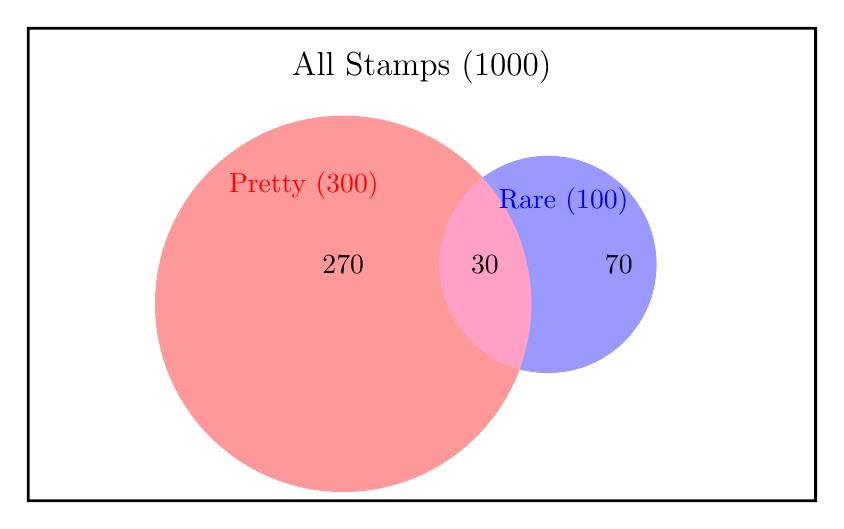
\begin{tikzpicture}
  \begin{scope}[blend group = soft light]
    \draw (-5, 3) rectangle (5, -3);
    \fill[red!40]  (-1, -0.5) circle (2.39);
    \fill[blue!40] (1.6, 0)   circle (1.38);
  \end{scope}
  \node       at (0, 2.5)    {\large All Stamps (1000)};
  \node[red]  at (-1.5, 1)   {Pretty (300)};
  \node[blue] at (1.8, 0.8)  {Rare (100)};
  \node       at (-1, 0)     {270};
  \node       at (2.5, 0)    {70};
  \node       at (0.8, 0)    {30};
\end{tikzpicture}
}
\caption{Venn diagram for the stamps example. The rectangle represents all the
  stamps, the large red circle represents the pretty stamps, and the small blue
  circle represents the rare stamps. The numbers indicate how many stamps are in
  each region.}
  \label{fig:stamps}
\end{figure}

Now let's simulate some data to further illustrate the problem. In this simulation,
we use the ``popular books whose movie adaptations were not-so-good'' example.

\showCode{R}{Code/datacollect-berkson.R} %
\runR{Code/datacollect-berkson.R}{datacollect-berkson} %

In the above code, the goodness of books and movies are drawn independently from a
standard normal distribution (\wingding{1} and \wingding{2}). \wingding{3}
checks if a book is good (better than 90\% of all books) and \wingding{4} checks
if a movie is good (better than 90\% of all movies). A component of the variable
\code{good} in \wingding{5} is \code{TRUE} if the book and/or the movie is good.
Running the above code should give the two figures in Figure~\ref{fig:berkson}
and the following output.
\includeOutput{datacollect-berkson} %

We see from the output and Figure~\ref{fig:berkson} (a) that the correlation between
the goodness of books and the goodness of movies is very close to zero---there
is no linear association between them. However, if we limit our data to inoclude
only movies such that either the book is good, or the movie is good, or both are good, 
and we then look for a linear association between the quality of books and movies,
then there is a clear negative linear relationship, as can be seen in 
Figure~\ref{fig:berkson} (b).


\begin{figure}[H]
  \begin{subfigure}{0.485\textwidth}
    \includegraphics[width=\textwidth]{images/chapter_6/berkson1.pdf}
    \caption{No linear association between goodness of movies and goodness of
      books}
  \end{subfigure}
  \begin{subfigure}{0.485\textwidth}
    \includegraphics[width=\textwidth]{images/chapter_6/berkson2.pdf}
    \caption{Negative linear association for top 10 percent books and/or movies}
  \end{subfigure}
  \caption{Goodness of movies v.s. goodness of books}
  \label{fig:berkson}
\end{figure}

People typically only recommend good books or good movies to other
people, so what we see are only these with the best review. If a book is
bad and the movie based on it is terrible, it's very likely that you ever have
a chance to hear about them. Thus, the impression that Hollywood ruins good books is
false. It's just an impression based on a biased sample. 

The `blank square' in the bottom-left corner of Figure~\ref{fig:berkson} (b), where we see no
points at all, is our \emph{dark data} in this example, and is the source of
our biased result, and the false impression. There are, in fact, many data
points in this region, but we never observe them. They include the majority of
bad books and bad movies.

This type of selection bias problem is related to the idea of \emph{conditional probability},
which we discussed in Chapter~\ref{ch:probability}. When we calculate probabilities, or
obtain other statistics, our results depend on the  set of possible events. If we limit 
the set of observable events, we should generally expect our selection to have
an impact on our analysis. Only when the selection of the subset is \emph{independent}
of the characteristics of subjects in the population, can we trust the results obtained
from a sample.

\hypertarget{ch:data}{%
\subsection{Survival Bias}\label{survival-bias}}

Survivor bias arises when observations are limited to subjects or objects that
have ``survived'' or successfully completed a particular process, while those
that did not are overlooked. For instance, poorly performing hedge funds often
close and are excluded from indexes, skewing performance analyses. Similarly,
prominent success stories like Facebook dominate the spotlight, overshadowing
the vast majority of failures. Ignoring survivor bias can result in misleading
or even entirely incorrect conclusions, as it fails to account for the unseen
data that play a critical role in understanding the complete picture.

\begin{example}[hit aircraft]
During World War II, aircraft that had returned from missions were examined and
the most-hit areas of the plane are given in
Figure~\ref{fig:survival-bias}. Which areas should the army add armor to
increase the survivorship of the planes?

A direct intuition may suggest to reinforce areas with the most bullet holes
because these are the most hit region. However, the data were collected from the
aircraft that had survived their missions, and if an aircraft was hit and down
it would not be included in the data. If there is a bullet hole in the engine
area or in the cockpit, then it would unlikely that the aircraft could
return. This was actually the reason why the engine and cockpit regions were
almost free of bullet holes. Knowing that the marked dots for bullets holes were
a biased sample and the cause of the bias, we should realized that these regions
with bullet holes could take damage and the aircraft could still fly well enough
to return safely. These regions did not need additional armor. It is the areas
where the returning aircraft were unscathed that need additional armor.
\end{example}

This example shows that ignoring the bias may give a very wrong conclusion. If
we take into account the source of the bias, then we can still obtain valid
result from a biased sample.

\begin{figure}[H]
  \includegraphics[width=.85\textwidth]{images/static/Survivorship-bias.png}
  \caption{Most-hit areas of the returned aircraft. Source: \url{https://en.wikipedia.org/wiki/Survivorship_bias}}
  \label{fig:survival-bias}
\end{figure}

\hypertarget{ch:data}{%
\subsection{Omitted Variables}\label{omitted-vars}}
Sometimes we just don't know that we're missing critical data. It can be
in the form of base-rate fallacy, where the data we may be ignoring
(unless we're careful) is the prevalence of something in the population,
such as blood type or a disease. In other cases, we may be missing data
because of \emph{selection bias}, where we inadvertently analyze only
a non-random sample, as was the case with Berkson's bias or in the
survival bias story.

If we think of the data as a table in which the rows are subjects (cases) and
the columns are variables---properties of each subject or case, then the previous
examples were all about missing \emph{rows} in the table. When
rows are missing completely at random, we can still get good estimates
and predictions, but if they are missing in some systematic way, then
the results we get can't be trusted. They may be biased and lead to wrong 
conclusions.

In this subsection we consider the case where what we're missing
is \emph{columns} (variables) in the data table.
We've already seen two such examples in previous chapters. The first one
appeared in Chapter~\ref{EDA}, Figures~\ref{sidebysidebp} and 
\ref{scatter}. There, the variables where \code{x} (e.g., time) and
\code{g} (e.g., the A/C is working or not). We saw that only when we 
considered both variables  \code{x}  and  \code{g}, were we able
to see the real pattern of \code{y} (say, the temperature).

The second example appeared in Chapter~\ref{simpsons-paradox}, where we
discussed Simpson's paradox. When we looked at the overall admission rate
to UC  Berkeley, it looked like the rate for women is considerably lower, but when 
we added a variable (the specific departments), the conclusion was quite different,
and in fact, in most departments the admission rate was higher for women.

The trouble with this kind of missing data is that we may never know what's missing!
As we discussed in Chapter~\ref{EDA}, we should always try to use plots and tables
to visualize and understand the nature of the data. In
Chapter~\ref{ch:regression} about \textcolor{red}{regression} 
we'll see that in some cases we may get hints for missing variables from the so-called
regression diagnostics plots.

\runR{Code/datacollect-omitted.R}{datacollect-omitted}

However, there's no guarantee that we'll be able to identify a missing variable, 
which may lead us to misinterpretations of data. To see it, let's look at another example.
Phil is a realtor who works in a small college town. The college has been around for
a couple of centuries, and is very prestigious. His clients often wonder
why the houses that are farther from the campus cost so much more than the 
ones in walking distance.
Phil collected data and plotted the graph in Figure~\ref{fig:omitted},
which shows the square of the distance in miles of houses from the 
campus on the x-axis, and the price (in thousands of dollars) on the 
y-axis. He also added a fitted line, which shows a positive trend.

\begin{figure}[H]
  \includegraphics[width=.6\textwidth]{images/chapter_6/omitted.pdf}
  \caption{The relationship between the square of the distance from a house to the campus, and 
  the house price, in thousands of dollars}
  \label{fig:omitted}
\end{figure}

Phil concludes that, indeed, the farther the house is from campus, the more
expensive it is. But surely, many people who work at the university prefer to
live close by and have the means to do so—so what could drive the prices of more
remote houses up?

With observational data, it's tempting for Phil (and most people) to find
a way to explain a phenomenon that defies common sense.
For example, Phil may come up with a theory that faculty want to
live away from campus in order to avoid their students. Or, he may 
hypothesize that close to the campus the crime rate may be higher than in the
suburbs. You can probably come up with other plausible explanations.
However, without additional information, they are just guesses. These guesses
may seem reasonable, but they are almost certainly wrong because,
after all, there are many more \emph{wrong} models than right ones (of 
which there may be just one, or it could be that what we observe is just
due to chance!)

In this case, we simulate the data, so we know the real reason. You can see
how we did it in the following code. In  \wingding{1} we create
an inverse relationship between the square root of the house age and
the distance from campus. (This is a simulation so we can do anything, 
but the motivation for this is that in reality, college town often expand around the 
campus.)

In  \wingding{2} we generate a linear relationship between the house price and
the distance to the campus. So, it seems like distance to campus is associated
with the price, as we show by fitting a model in \wingding{3} with the \code{lm}
function, but in fact, the distance is itself determined by age. So, in this
story, old houses cost less than new ones, but they are also closer to the college
for historical reasons. If we only consider distance, we'll miss the relationship
between price and the age of a house.

\showCode{R}{Code/datacollect-omitted.R}

This story also demonstrates another common pitfall, called \emph{confirmation bias}.
When we use observational data and see an interesting relationship, it's natural
to come up with an explanation. Once we do that, we may say: `oh, yes, that makes sense!'
even though before looking at the data we had a totally different idea in mind.
The `it makes sense' argument is not a valid scientific method to prove or
disproves theories!

This is often a subconscious process. Once we see some phenomenon or
relationship, we start seeking explanations and data that will support our
perception, and often also ignore data not supporting it. Finding the right
explanation or model may not be possible, but we must be aware of the 
possibility that ours is wrong. Establishing causality is generally impossible
with observational data, and we have to remember the risk of confirmation bias.


\hypertarget{ch:data}{%
\subsection{Extrapolations}\label{extrapolations}}

One of the main reasons to collect data is so that we can make predictions.
It allows us to use historical data to, for example, decide whether to take 
an umbrella when we leave the house, or how long it would take us to
get to our destination, given the traffic and our speed.

\runR{Code/datacollect-extrapolate.R}{datacollect-extrapolate}

Look at Figure~\ref{fig:ext1}, which shows the relationship between \code{x}
and \code{y}, for \code{x} between 0 and 0.25. We've also added the line
\code{y=x} for reference. Can you guess the value of \code{y} when \code{x}=0.5? 
How about  when \code{x}=2?

\begin{figure}[H]
  \includegraphics[width=.6\textwidth]{images/chapter_6/extra1.pdf}
  \caption{The relationship between \code{x} and \code{y}}
  \label{fig:ext1}
\end{figure}

Did you guess that when  \code{x}=0.5, \code{y} will be approximately 0.5, 
and when  \code{x}=2, \code{y} will be approximately 2?
This is a reasonable guess based on the data that we have, but is it true?

Let's see how to answer it with the following simulation.
In \wingding{1}, we generate 500 values for \code{x}, equally spaced 
between 0 and 2. Then we generate random errors in \wingding{2}, which
we call \code{e}.
Next, we generate three functions: in \wingding{3} we create a linear
function of \code{x}, in \wingding{4} we create the function \code{log(1+x)},
and in \wingding{5} and \wingding{6} we generate an exponential function that
increases between 0 and 1, and decreases after 1.
The three functions are shown in Figure~\ref{fig:ext2}.

\showChunk{R}{Code/datacollect-extrapolate.R}{EXT1}

In the range shown as a rectangle (for \code{x} between 0 and 0.4), the three functions are
nearly identical.
However, beyond 0.4, the three functions become very different. While \code{y1}
continues along a straight line,  \code{y2} starts to `bend' and although it continues to
increase, it does so at a slower rate. The function \code{y3} increases at an exponential
rate at first, but then it has a change-point, where the trend changes and it starts to decrease.

\begin{figure}[H]
  \includegraphics[width=.6\textwidth]{images/chapter_6/extra2.pdf}
  \caption{The relationship between \code{x} and \code{y} for three different function. Between
  0 and 0.4, the three functions are similar, but after that they are different}
  \label{fig:ext2}
\end{figure}

The code used to produce  Figure~\ref{fig:ext2} is as follows. Note that we
show a sample of 100 points out of the 500 (using the variable \code{pts}),
only to make it easier to see individual points.

\showChunk{R}{Code/datacollect-extrapolate.R}{EXT2}

What this example shows is that it's not possible to get reliable predictions beyond the
range of the data. In other words, if we try to extrapolate and extend our predictions
to values that were not observed in our sample, we may be way off! There's no
way to tell how the function we try to predict behaves outside the range
of observed \code{x}.

It is possible to perform a follow-up experiment, and check if our prediction is
correct. For example, suppose that \code{y} in the data in Figure~\ref{fig:ext1}
represents the average monthly amount spent on online shopping in thousand of dollars,
and \code{x} represents their annual income (in \$100,000). In our original sample
which gave us Figure~\ref{fig:ext1}, we only had people who spend between 0 and \$300
in a month, and their annual salaries were between 0 and \$30,000, with an
approximate linear relationship between \code{x} and \code{y}.

If we want to know the spending habits of people with higher income, we could
perform a second study and collect data for people who make \$50,000, \$100,000,
\$150,000, and \$200,000, and see how much they spend each month on online shopping, 
and see whether the linear trend continues, or whether a different function
fits better when we look at an extended range of \code{x} values.


\hypertarget{ch:data}{%
\subsection{Aliasing}\label{aliasing}}
\runR{Code/datacollect-aliasing.R}{datacollect-aliasing}
Suppose that we have data that we know consists of periodic functions.
This is very common in time series data for temperatures, for example.
It is also very common in signal processing. For example, music that
we hear on the radio or some streaming service is transmitted as combination
of frequencies, which can be represented with the sine or cosine functions.
The higher the frequency, the more high-pitch the sound. People can hear
a range of frequencies, up to a few thousand oscillations per second.

Let's generate some data, and try to estimate the true function from it
using the following code. Don't worry for now about  \wingding{1}, where
we initialize the parameter \code{f}. We'll get back to it later.
We start by choosing a small time interval in \wingding{2}, and 
divide the interval $[0, 3]$ into equal parts in  \wingding{3}.
In  \wingding{4}, we get the sample (e.g., by measuring the temperature,
or the frequency of some sound).
We show a  plot of the data in the left panel
of Figure~\ref{fig:aliasing1}. 

\why{Some variables such as dt1, \code{dt1_est}, and dt2 are used only one
time. Maybe remove them to shorten the code?}
\showChunk{R}{Code/datacollect-aliasing.R}{aliasing1}

We know that the data is supposed to be of the form
$$y(t)=\cos(2\pi ft)\,,$$
for some unknown frequency $f$. So, we use the  code in
\why{\wingding{5}-\wingding{7}?} \wingding{5} and \wingding{5}  to interpolate the data at more dense,
and equally spaced points. For the interpolation, or fitting the data, 
we use the function \code{interp1} from the \code{pracma} package.
We can see  in the right panel of  Figure~\ref{fig:aliasing1} that the 
interpolated function fits the data perfectly.

But, is it really a perfect fit?

\begin{figure}[H]
  \includegraphics[width=\textwidth]{images/chapter_6/aliasing1.pdf}
  \caption{Sampling from a periodic function, with a low sampling rate}
  \label{fig:aliasing1}
\end{figure}

 
In the data that we collected we have only $n=31$ samples. Let's try to
obtain a larger sample. Again, it will be evenly spaced, but our new sample
will be 10 times larger.
Let's look at the following code:

\showChunk{R}{Code/datacollect-aliasing.R}{aliasing2}

As you can see in \wingding{1}-\wingding{4}, we now collect data for
our sample at a rate that is 10 times higher than before (it's the same code
as before, except that the time intervals are 0.01, instead of 0.1). In \wingding{5} 
we plot the data that we got from the first (low sampling rate) data.
The new function is shown in Figure~\ref{fig:aliasing2}, and it also fits perfectly.

\begin{figure}[H]
  \includegraphics[width=0.5\textwidth]{images/chapter_6/aliasing2.pdf}
  \caption{Sampling from a periodic function, with a high sampling rate}
  \label{fig:aliasing2}
\end{figure}

How can it be? Which function is the correct one? What we see here is, that
for different sampling rates we get different fitted functions, and all of them
can fit the data perfectly. This phenomenon is called \emph{aliasing}.

Can we tell which one is correct? In general, when fitting functions, the answer
is no. However, when dealing with data which is a mixture of periodic functions
the answer is yes! We should sample at equally spaced points, so that
the total number of points is twice the highest possible frequency (number of 
oscillations per time unit.)
We can sample more frequently, but we will not gain anything. This sampling rate is
optimal---no smaller one is sufficient, and a larger one is not needed.

Let's revisit the parameter \code{f} which we saw in \wingding{1}. This is
the true frequency that we used. What it means is, that we know the
function has to oscillate 8 times per time unit. Now, look at Figures  
\ref{fig:aliasing1} and \ref{fig:aliasing2}. Can you tell which one is the correct 
function? The function in Figure~\ref{fig:aliasing1} completes only two
cycles between 0 and 1, while the one in Figure~\ref{fig:aliasing2}
shows 8 cycles in one time unit. The higher sampling rate gave us the
true function. The lower sampling rate, although fits the given data perfectly, 
gives us the wrong function.

So, when dealing with data like in this example, it's important to have some prior
knowledge about the maximum possible frequency. In the case of temperature data,
we know that the data has a roughly cyclical shape, with one cycle per 
year. For audio data, the average person hears sounds that are composed of
waves that oscillate around 4,000 times per second. (Dogs, for example
can hear much higher frequencies). So, a telephone only has to sample the
audio at a rate of 8,000 times per second.

We mentioned in Section \ref{representative} of this chapter that a representative sample is more
important than a large sample, but here we see that in some situations
the sample size is also important. In the examples discussed here,
we know exactly how large the sample has to be in order to identify
the correct function, and prevent the problem of aliasing.



\hypertarget{ch:data}{%
  \section{Common biases}\label{sources-bias}}
We've seen a number of sources of bias above, including Berkson's bias---where
we only get to observe data based on some selection rule,
the related survival bias---where we never see the outcome from the worst case 
scenario, the base-rate fallacy---where ignoring the prevalence of some
condition in the entire population leads to wrong conclusions, and
bias due to omitted variables.

There are other sources of bias. Some of them are hard to prevent,
but being aware of the potential problems is an essential step
before we do any analysis. Here are a few examples.

Some biases are due to human tendencies. For example, \emph{observation time
interval bias} may occur if data collection ends too early, or worse, when it is
stopped at a convenient time that supports the desired conclusion.

\emph{confirmation bias} occurs when people
try to search for, interpret, favor, and recall information in a way that confirms
or supports their prior beliefs or values. It's also sometimes referred to
as \emph{cherry picking}.  The picker selects only the ripest and most
appealing fruits, and the collection is not representative of all the fruit in the 
orchard. 

Another example is \emph{availability bias}, which arises because
people have a natural tendency to assign probability or likelihood
to events based on how easily they can recall them. Exposure to news
items can lead to this type of bias. Topics that receive a lot of media
attention (such as disease diagnoses or disasters)
tend to stay on people's minds, leading to overestimation
of their actual probabilities.

Even when data are collected in a carefully designed experiment, some bias may occur.
For example, rejection of bad data on arbitrary grounds instead of according to
a previously stated or generally agreed criteria. For example, one may choose
to discard what one perceives as ``outliers'' without valid reasons.

Another common source is \emph{self-selection bias} or a \emph{volunteer bias},
which happens when subjects in an experiment decide on their own if they will be included in a
sample, or in each group in the sample. Volunteers tend to have intrinsically different characteristics from
the whole population of people in consideration. 
For example, people with a terminal disease are much more likely to opt into
a clinical trial of an experimental drug. If only terminally ill patients receive the
treatment, then we wouldn't be able to tell if it works or not. It may look like
it doesn't work, but this may be true only for people who are about to die, but
if the treatment is applied at an earlier stage, it may be very effective!
  
Surveys may suffer from \emph{nonresponse bias} which is caused by subjects 
not answering specific questions. This may happen more often with
personal or sensitive questions.
Related to this is the ``Hawthorne effect'', which is when people tend to behave
differently if they know they're being observed.
This one is particularly hard to detect or to prevent.

\hypertarget{ch:data}{%
  \section{Basic sampling designs}\label{sampling-designs}}

Sampling can be conducted with or without replacement. Sampling with replacement
may produce duplicate selections (e.g., the birthday problem in
Chapter~\ref{ch:probability}) but is often simpler to implement. Sampling
without replacement avoids duplicates and yields higher precision, especially
when sampling a large proportion of the population.

There are various sampling designs, and the best choice depends on the
population, research objectives, and available resources. Below are some basic
sampling designs. Most advanced sampling methods are built by combining these
foundational designs in various ways.
\begin{itemize}
  
\item Simple Random Sampling: Every element in the population has an equal
  chance of selection, typically using random numbers or a lottery. This method
  is straightforward and minimizes sampling bias, but may be impractical for
  large or hard-to-access populations and can result in high sampling
  variability. It is best suited for small accessible populations.

\item Stratified Sampling: Divide the population into homogeneous subgroups
  (strata), then select a simple random sample from each stratum. This ensures
  representation from all subgroups and increases precision, making it
  especially useful for heterogeneous populations. However, it requires detailed
  population information and careful definition of strata to avoid bias.

\item Systematic Sampling: Select every \(k\)th element from a list after a
  random starting point. This method is simpler and more efficient than random
  sampling, and ensures samples are evenly spread through the
  population. However, it may introduce bias if a pattern exists in the list.

\item Cluster Sampling: Divide the population into clusters (e.g., geographic
  areas), randomly select some clusters, and sample all or some items within
  them. This method is cost-effective for large, geographically dispersed
  populations, but typically results in higher sampling error compared to other
  designs.

\item Weighted Sampling: Assign higher selection probabilities to more
  informative or important elements. This method can improve estimation
  efficiency when elements vary in informativeness, but generally yields biased
  samples that require specialized estimation techniques. It also relies on
  population information and appropriate weights, which may not always be
  available.
\end{itemize}




% \hypertarget{ch:data}{%
%   \section{Different sampling approaches}\label{sampling-approaches}}
% %%%%----------------------------------------------------------
%   \begin{itemize}
%   \item Sampling with replacement: An element may be included in a sample more than once. It is possible to have replicates in the sample.
%   \item Sampling without replacement: An element can be included in a sample at most once. There is no replicates in the sample.
%   \item Poisson sampling: determines if each element of the population is selected in the sample independently. The sample size is random.
%   \item Between Sampling with replacement and without replacement, which is more efficient?
%   \end{itemize}

% %%%%----------------------------------------------------------
% \begin{example}[Numerical comparisons]
%   \begin{itemize}
%   \item To simulation hosehold incomes, generate a population P of size $N$ from a $P\sim\chi^2$ distribution with degrees of freedom one.
%   \item Take samples of size $n$ from P to estimator the population mean, say $\mu$, using simple random sampling both with and without replacement. Compare their efficiency.
%   \item Assume another variable $A=P+Unif(0,2)$ is available to define informative sampling weights. Evaluate the efficiency of weighted sampling both with and without replacement. 
%   \end{itemize}
% \end{example}

\section{Summary}
In this chapter we discussed the importance of proper sampling, and the risk of 
reaching wrong conclusions when the data collection is not done
right. We introduced the notion of a representative sample, and demonstrated
what can happen when a sample is non-representative (biased).
In general, when the data collection is done as a planned experiment,
we can prevent biases (but it's still not always easy, and require careful planning!)
But, when we use so-called observational data, there is not much we can do to
prevent bias in data collection. We should, however, be aware of the possible
biases, and be careful not to draw far-reaching or decisive conclusions when
we can't be sure that there is no hidden bias.

%%% Local Variables:
%%% mode: latex
%%% TeX-command-extra-options: "-shell-escape"
%%% TeX-engine: xetex
%%% TeX-master: "../sidsmain.tex"
%%% End:

%\chapter{Hypothesis Testing}
\label{ch:hypothesis}

Life is full of decisions where we don’t know the truth but still need
to act. Is that coin you’re flipping really fair, or does your sneaky
friend always seem to win the toss? Should you trust that online
review saying pineapple pizza is amazing, or was it written by someone
with questionable taste? In situations like these, we’re left making
judgments without ever being 100\% sure of the answer. Hypothesis
testing is the scientific version of this everyday decision-making
process. It’s not about proving something beyond all doubt; it’s about
weighing the evidence and making the best call with the information at
hand---like a courtroom verdict, but with fewer objections and more
statistics.


\section{Basic Concepts}

Hypothesis testing formalizes how we handle uncertainty in data-driven
decisions. In practice, we ask questions like: Is a new drug effective
in treating a disease, or is it no better
than the current standard? Is one commercial more effective than another 
in driving sales on a website (a process often referred to as an A-B test)? 
Can the observed increase in global mean temperature be attributed to human 
activities? Or, is the 30-day hospital readmission rate higher among minority 
patients compared to others?


At the core of hypothesis testing lies a simple setup. There are two 
competing explanations: the
\emph{null hypothesis}\index{\emph{null hypothesis}},
$H_0$, which represents
the default position or baseline assumption, and the
\emph{alternative hypothesis}\index{\emph{alternative hypothesis}},
$H_1$, which reflects a meaningful difference or effect.
In the new drug example, $H_0$ states that the drug has no effect, 
while $H_1$ claims it does. Depending on context, $H_1$ may represent
the investigator's belief, but not necessarily what they hope to 
support---sometimes the goal is to rule out harm or demonstrate
equivalence.


Think of hypothesis testing as a strategic game. Nature knows the
truth---whether $H_0$ or $H_1$ is correct---but keeps it hidden. Our
job is to examine the available evidence from the observed data and
decide which hypothesis to accept. This process is not
foolproof; we might reject $H_0$ when it is true
(a \emph{Type~I error}\index{\emph{Type~I error}}), or fail to 
reject $H_0$ when $H_1$ is true (a \emph{Type~II error}\index{\emph{Type~II
    error}}). Understanding and managing these risks is fundamental part
of hypothesis testing and highlights both its challenge and nuance.


\subsection{Stochastic Analog of Proof by Contradiction}

Hypothesis testing can be viewed as a stochastic analog of proof by 
contradiction \citep{reeves1980hypothesis}. In mathematics, proof by
contradiction starts by assuming
the negation of the statement we wish to prove. Logical reasoning then
leads to a contradiction, thereby establishing the original 
statement to be true. Similarly, in hypothesis testing, we start by 
assuming the null hypothesis, $H_0$, is true and assess
whether the observed data align with this assumption. If the data 
deviate from what we would expect under $H_0$ to a sufficient degree,
we reject it in favor of the alternative hypothesis, $H_1$.


Despite the shared structure--- both approaches begin with an
assumption and seek evidence that undermines it---there is a
fundamental difference. Proof by contradiction yields logical
certainty, while hypothesis testing is inherently probabilistic.
Rejecting $H_0$ does not definitively prove $H_1$; instead, 
it means the evidence against $H_0$ exceeds a pre-specified threshold
to favor $H_1$. Similarly, failing to reject $H_0$ does not confirm
its validity, only that the data do not provide sufficient grounds for 
rejection.


\subsection{Type~I and Type~II Errors}

The probabilistic nature of hypothesis testing introduces two types of 
decision errors. A \emph{Type~I error}\index{\emph{Type~I error}}
occurs when we reject the null hypothesis, $H_0$, even though it is
true. This is often referred to as false positive, the incorrect
conclusion that an effect exists when it actually does not.
The probability of making this error is called the \emph{significance
  level}\index{\emph{significance level}}, denoted by $\alpha$. A
smaller~$\alpha$
reduces this risk but may make it harder to detect real effects.
A \emph{Type~II error}\index{\emph{Type~II error}} arises when we fail to
reject $H_0$ even though it is false. This is often referred to as
false negative error, reflecting the risk of missing a true effect,
with its probability denoted by $\beta$. The quantity $1 - \beta$,
called the \emph{power}\index{\emph{power}} of the test, masures the test's
ability to detect an effect when one truly exists.


\begin{example}[Lady testing tea]
R. A. Fisher's ``Lady Tasting Tea'' experiment, described in his 1935 
book \emph{The Design of Experiments} \citep{fisher1935design},
became one of the earliest and 
most elegant demonstrations of formal hypothesis testing 
\citep{salsburg2002lady}. Fisher recounted an event at Rothamsted 
Experimental Station, where a colleague claimed she could tell by 
taste whether milk or tea had been poured first into a cup. To test 
this claim, Fisher designed an experiment involving eight cups of tea: 
four prepared with milk poured first, and four with tea poured first. 
The cups were presented in random order, and the lady was told that 
there were four of each kind. Her task was to identify the four cups 
with milk poured first. Assuming the null hypothesis, $H_0$, that she 
was guessing, Fisher calculated the probability of her achieving a 
result as good as the observed one purely by chance.


If her performance was highly unlikely under $H_0$, the null hypothesis 
would be rejected in favor of the alternative, $H_1$, suggesting she 
may truly have the claimed ability. This decision, however, carried the 
risk of a Type~I error---concluding she had the ability when she did 
not. Conversely, failing to reject $H_0$ could result in a Type~II 
error---overlooking a genuine ability due to insufficient evidence. The 
experiment highlighted how statistical decisions are made under 
uncertainty and how error probabilities---Type~I and Type~II---must be 
considered in the design and interpretation of hypothesis tests.
\end{example}


\subsubsection{Test Statistic and P-Value}

In hypothesis testing, a \emph{test statistic}\index{\emph{test statistic}} 
is a numerical summary of the data used to evaluate the null hypothesis, 
$H_0$. It captures the relevant aspects of the observed data under 
$H_0$ and quantifies the evidence against it. The choice of test 
statistic depends on the specific hypothesis and the structure of the 
data. A test rejects $H_0$ if its test statistic, denoted by $T$, 
falls into a designated \emph{rejection region}\index{\emph{rejection region}}. 
The probability that $T$ falls in this region when $H_0$ is true is 
called the \emph{significance level}, typically denoted by $\alpha$. 
This threshold is usually chosen to be small, such as 0.05 or 0.01, 
to limit the chance of making a Type~I error.


The \emph{p-value} provides an alternative way to summarize results. 
It is defined as the probability, under $H_0$, of obtaining a test 
statistic as extreme as or more extreme than the observed one. A small 
p-value indicates that the observed result would be rare under $H_0$, 
thus providing evidence against it. The decision rule is simple: 
if the p-value is less than $\alpha$, we reject $H_0$; otherwise, we 
fail to reject it. This offers flexibility, as the same p-value can 
be compared against different significance levels depending on
context.


The p-value is often misunderstood as the probability that $H_0$ is 
true given the data. This is incorrect. The p-value assumes that 
$H_0$ is true and measures how surprising the observed data are under 
that assumption. As shown in empirical studies, this misinterpretation 
is widespread, even among statistically trained researchers 
\citep{falk1995significance}. Understanding that the p-value reflects 
compatibility between the data and the null model---not the truth of 
the hypothesis---is essential for proper statistical reasoning.


\begin{example}[Lady tasting tea (continued)]

In the Lady Tasting Tea experiment, the test statistic $T$ is the 
number of cups the lady correctly identifies as having been prepared 
with milk poured first. The total number of cups is an even number $n$, 
with exactly $n/2$ prepared milk-first and $n/2$ tea-first. Importantly, 
the lady is told in advance that there are exactly $n/2$ of each type, 
and she is required to label exactly $n/2$ cups as milk-first. Under the 
null hypothesis $H_0$, she is assumed to be guessing. In this setup, 
it can be shown that the distribution of $T$ under $H_0$ follows a 
\emph{hypergeometric distribution}\index{distribution!\emph{hypergeometric}}, 
and large values of $T$ provide stronger evidence against $H_0$.


To carry out the test, we fix a significance level $\alpha$, such as
$0.05$, representing the maximum tolerable probability of a Type~I
error. We then define the \emph{rejection region}, consisting of
values of $T$ that are considered too extreme to plausibly occur under
$H_0$. Suppose we choose $\{n/2\}$ as the rejection region—that is, we
only reject $H_0$ if the lady achieves a perfect classification. The
probability of this outcome under $H_0$ is
$\Pr(T = n/2) = 1 / \binom{n}{n/2}$.


For example, suppose $n = 8$ and the lady correctly identifies all 
$4$ milk-first cups. The observed test statistic is 
$T_{\text{obs}} = 4$, and the p-value is 
\[
  \Pr(T \ge T_{\text{obs}} \mid H_0) = 1 / \binom{8}{4}
  = 1/70 \approx  0.0143.
\]
Since this p-value is smaller than the commonly used significance
level $\alpha = 0.05$, we would reject $H_0$ and conclude that her
performance is unlikely to be due to guessing.


Now increase the number of cups to $n = 10$, with the lady again 
achieving a perfect identification of the $5$ milk-first cups. The 
p-value is
\[
  \Pr(T \ge 5 \mid H_0) = 1 / \binom{10}{5}
  = 1 / 252 \approx 0.0040.
\]
This smaller p-value gives even stronger evidence
against~$H_0$---suggesting that her performance is highly unlikely to
be the result of chance guessing and that she may indeed have the 
ability to tell the difference.
\end{example}

\section{Permutation Tests}

The test we performed in the example of lady tasting tea belong to a
general family of tests known as the
\emph{permutation test}\index{test!permutation}.

\subsection{Permutation under Exchangeability}

A permutation test relies on the assumption that under the null
hypothesis~$H_0$, certain labels indicating the groups of the data are
exchangeable. This means that if $H_0$ is true, the observed values in
different groups come from the same underlying distribution, and any
difference across groups is due to random variation.
As such, the extremeness of the observed test statistic
can be assessed with the same testing statistics calculated on all
randomly permuted versions of the observed data.


By pooling all the data and randomly reassigning the group labels, we 
simulate what the data might look like if $H_0$ were true. Each 
permutation represents a potential arrangement of the data
under~$H_0$, and the distribution of the test statistic across these
permutations forms the \emph{sampling distribution under
  $H_0$}\index{sampling distribution!under $H_0$}. Comparing the
observed test statistic to this distribution allows us to calculate its
p-value, which quantifies how extreme the observed result is
under~$H_0$.


For instance, in the ``Lady Tasting Tea'' experiment, the null hypothesis 
$H_0$ assumes that the lady is guessing randomly. Under this assumption, 
all possible arrangements of the cups are equally likely, making the 
permuted sampling distribution an exact representation of $H_0$.
Similarly, when testing for a difference in means between two groups,
which could, for example, be a treatment group and placebo group in a
clinical trial setting. The distribution of the difference in two
group means when the groups are randomly permuted reflects the
behavior of the test statistic when there is no true difference
between the groups.


In some scenarios, the total number of possible permutations can be
too large, making it prohibitive to exhaust all permutations to form
exact sampling distribution. 


\subsection{Monte Carlo Approximation}

When it is infeasible to exhaust all possible permutations, we can use
Monte Carlo approximation to draw a large number of possible
permutations, and approximate the sampling distribution based on
empirical distribution of the test statistic computed from this large
number of random permutations.

\begin{example}[Familial clustering of certain diseases]
\runR{Code/hypo-familial.R}{hypo-familial}

Consider a study of 10 families, each with 4 relatives participating.
Each person either shows a certain symptom (coded 1) or not (coded 0).
We want to test whether the symptom tends to appear in clusters within
families. In other words, do relatives share the symptom more often
than would occur by chance?

Here is what the data looks like:
\showChunk{R}{Code/hypo-familial.R}{dataHead}

Consider a testing statistics $T$ which is defined as the total number
of within-family concordant pairs. Here a concordance pairs mean 1-1
pairs.

\showChunk{R}{Code/hypo-familial.R}{familyStat}

Under the nyull hypothesis that there is no familial clusterin
of this symptom, we can randomly permute the symtom lalel across all
individuals across the families. For each permutation we can compute
the total number of within-family concordant pairs. The empirical
distribution of this count gives us the basis to assess whether the
observed $T$ is overly extreme or not. The p-value is approximated by
the proportion of such $T$ that are as extreme or more extreme thatn
the observed version.

\showChunk{R}{Code/hypo-familial.R}{familyPvalue}


We apply the functions to the example dataset and get the observed
testing statistic and its p-value.

\showChunk{R}{Code/hypo-familial.R}{application}
\end{example}

\begin{example}[Permutation test for two-group comparison]
To make this concrete, let us consider a two-group comparison
example. Suppose we have two
groups of data, $x_1$ and $x_2$, with sample sizes $n_1 = n_2 = 30$. 
If $H_0$ is true, there is no real difference between the groups, so 
the observed difference in the sample means, $\bar x_1 - \bar x_2$,
where $\bar x_1$ and $\bar x_2$ are, respectively, the sample mean of
the 1st and 2nd groups, is simply due to chance.

\showChunk{R}{Code/hypo-perm.R}{HypoPermSetup}

Here, \code{xd} is the observed difference in means between $x_1$ and 
$x_2$. Under $H_0$, which assumes no difference between the groups, 
any observed difference is due to random variation.


When we randomly shuffle the pooled data \code{$x_1$ and $x_2$} 
and split it into new groups of size $n_1$ and $n_2$, the resulting 
groupings represent plausible outcomes under $H_0$. Repeating this 
permutation many times allows us to build the sampling distribution 
of the test statistic under the assumption of no group differences.


To compute the p-value of the observed test statistic \code{xd},
we need the \emph{sampling distribution} of the test 
statistic under $H_0$. Permutation testing constructs this distribution 
by repeatedly shuffling the data to simulate the null hypothesis. For a 
single permutation, we shuffle the combined data, split it into two groups, 
and compute the test statistic:
\showChunk{R}{Code/hypo-perm.R}[HypoPermOnePerm]


Each permutation represents a possible arrangement of the data
under~$H_0$. The totle number of permutations is:
\showChunk{R}{Code/hypo-perm.R}[HypoPermFullCount]

This total number of permutations is about $1.18 \times 10^{17}$,
which is too large to exhaust. So we approximate the sampling
distribution using a subset of random permutations.
This is implemented in the following function:
\showChunk{R}{Code/hypo-perm.R}[HypoPermMyPermTest]

This function simulates \code{nperm} permutations, calculates the test 
statistic for each, and compares them to the observed test statistic to 
compute the p-value.


Let us apply the permutation test to two samples drawn from gamma 
distributions, with a true difference ($\delta = 10$):
\showChunk{R}{Code/hypo-perm.R}[HypoPermDemo]


This outputs the p-value, which quantifies the probability of observing a 
test statistic as extreme as or more extreme than the observed statistic 
under $H_0$. 
\end{example}


Permutation tests rely on minimal assumptions, making them robust to 
non-standard data distributions. The resulting p-value provides evidence 
against $H_0$: a smaller p-value indicates stronger evidence that the 
observed difference in means is not due to chance. By using random 
permutations, we efficiently approximate the sampling distribution when 
enumeration of all permutations is computationally infeasible.


\section{Properties of Hypothesis Tests}


\subsection{Properties of Hypothesis Tests}

Hypothesis tests are evaluated using two critical 
properties: their size, or significance level, and their 
power. These properties help us understand the reliability 
and sensitivity of a test in different scenarios.

The \emph{size} of a hypothesis test, also referred to 
as the \emph{significance level} and denoted by $\alpha$, 
is the probability of committing a \emph{Type~I error}. A 
Type~I error occurs when the null hypothesis, $H_0$, is 
rejected even though it is true. For instance, if $\alpha = 0.05$, 
there is a 5\% chance of falsely rejecting $H_0$ when it 
is true. This level is usually chosen in advance to control 
the risk of false positives, with typical values being 0.05 
or 0.01. Importantly, the size of a test depends on the 
sampling distribution of the test statistic under $H_0$. 
Tests that control their size consistently are said to 
be valid.

The \emph{power} of a test measures its ability to detect 
a true effect when one exists. It is defined as the 
probability of correctly rejecting $H_0$ when the 
alternative hypothesis, $H_1$, is true. Mathematically, 
the power is $1 - \beta$, where $\beta$ is the probability 
of committing a \emph{Type~II error}—failing to reject $H_0$ 
when $H_1$ is true. Higher power indicates greater 
sensitivity of the test to detect differences or effects, 
which is desirable in most applications. The power of a 
test depends on several factors, including the sample 
size, the true effect size, the significance level $\alpha$, 
and the variability in the data. Larger sample sizes, 
larger effect sizes, and smaller variability all contribute 
to higher power.

When two tests both maintain the same size, the one with 
higher power is preferred because it provides greater 
evidence against $H_0$ when $H_1$ is true. However, 
there is an inherent trade-off between size and power. 
Reducing $\alpha$ decreases the likelihood of Type~I 
errors but may increase the likelihood of Type~II errors, 
leading to lower power. Conversely, increasing power often 
requires relaxing the significance level or increasing 
sample size, which may not always be feasible.

In the next example, we will illustrate these 
concepts by comparing two common tests for comparing two 
samples: the t-test and the Wilcoxon test. Using simulations, 
we will examine their size and power under different 
conditions and demonstrate how their performance varies.


\begin{example}{Two-sample comparison}
First, let’s see how we can perform the tests for one pair of datasets:
\showCode{R}{Code/hypo-2samp.R}[2][9]


Here, \code{x1} and \code{x2} represent two groups of data. The t-test assumes
the data are normally distributed, while the Wilcoxon test is
distribution-free, meaning it works for a wider range of data
distributions.


Next, we create a function \code{do1rep()} that simulates one
experiment. This generates two groups of data, applies both tests, and
records their p-values.
\showCode{R}{Code/hypo-2samp.R}[13][22]


Here, \code{delta} represents the true difference between the means
of the two groups. When \code{delta = 0}, there’s no real difference
(null hypothesis is true). For each test, we calculate the p-value to
assess whether to reject the null hypothesis.

To evaluate the sizes (false positive rates) of the tests, we simulate
multiple experiments where \code{delta = 0} and calculate the proportions of
times the tests reject $H_0$.
\showCode{R}{Code/hypo-2samp.R}[26][28]

The function \code{rowMeans(sim < 0.05)} calculates the fraction of
times the p-value is below 0.05, representing the rejection rate for
each test.


We wrap the simulation into a function \code{empRejRate()} to
compute rejection rates for different sample sizes, distributions, and
effect sizes:
\showCode{R}{Code/hypo-2samp.R}[32][35]

Now, we compare the performance of the t-test and Wilcoxon test for
data from different distributions (normal and Cauchy):
\showCode{R}{Code/hypo-2samp.R}[38][44]

For the Cauchy distribution, which has heavier tails than the normal
distribution, the performance of the tests may differ significantly.


Finally, we compute and plot the power of the tests as the effect size
(\code{delta}) increases:
\showCode{R}{Code/hypo-2samp.R}[47][62]

These plots show the empirical rejection rates (power) as \code{delta}
increases. For the t-test, performance depends on the assumption of
normality, while the Wilcoxon test is more robust under non-normal
distributions like the Cauchy.
\end{example}

\section{Multiple Testing}

When we test one idea, we usually know what a ``significant result''
means. But what happens if we test many ideas at once? Does a small
p-value still carry the same meaning? Let us find out by running our own
simulations.

\begin{example}[20 Ineffective Drugs]
We begin with a simple story: a laboratory screens 20 new drugs to
see whether any of them improves a health score compared with a
placebo. Unknown to us, none of the drugs actually works. By
simulating this world, we can watch what happens when we run many
independent tests in parallel.


We first write a function that performs one full screening round,
returning 20 p-values from 20 two-sample t-tests.
\showChunk{R}{Code/hypo-multiple.R}{do1screen}


Even though all drugs are useless, some p-values will be surprisingly
small. To understand this more systematically, let us repeat the entire
screening many times.
\showChunk{R}{Code/hypo-multiple.R}{pvalues}


A histogram provides a clear view of the behavior of p-values under pure
noise:
\showChunk{R}{Code/hypo-multiple.R}{hist}

The shape is roughly flat, as expected when every null hypothesis is
true. But the more interesting question is: How many ignificant
drugs appear in each experiment?

Let us count how many of the 20 p-values fall below 0.05 in each
experiment.
\showChunk{R}{Code/hypo-multiple.R}{sigcount}

Although all 20 drugs are useless, most experiments still produce one or
two “significant” hits. In fact, the chance of seeing at least one
false discovery is high:
\showChunk{R}{Code/hypo-multiple.R}{meansig}


This number is typically around 0.64. In fact, when testing 20 useless
drugs at the 0.05 level, there is a $1 - 0.95^{20} \approx  64\%$
chance that at least one appears significant by accident.


This is one of the core issues of multiple testing.
\end{example}

% The Smallest P-Value Always Looks Exciting


Every experiment has a ``best'' drug, the one with the smallest p-value.
Let us look at that distribution.


Tiny p-values (like 0.01 or 0.005) appear quite often---even though
nothing is real. This does not mean the minimum p-value is useless;
indeed, there is a long history of using extreme values such as the
smallest p-value as a valid test statistic, provided we take into
account how many tests were performed.


The problem arises when we look at many tests, take the smallest
p-value, and then interpret it as if it came from a single test. In
that naive view, we are ignoring the fact that we gave ourselves many
chances to see something ``exciting.''


% What if some drugs actually work?

Now let us simulate a world where 4 out of 20 drugs truly have an
effect.


We compare two strategies:

1. Uncorrected testing: $p < 0.05$
2. Bonferroni correction: $p < 0.05/20$

We simulate many experiments and count true positives (TP) and false
positives (FP).


Uncorrected tests find many real effects but also many fake ones.
Bonferroni greatly reduces false positives, but also misses some real
drugs. The simulation reveals a simple trade-off:

Reducing false discoveries often reduces real discoveries too.



From these experiments, we discovered:
\begin{itemize}
\item A p-value only behaves as expected when we test one idea.
\item When we test many ideas, small p-values appear even if nothing is
  true.
\item The question ``What is the chance that at least one test shows
  significance?'' becomes central.
\item Adjustments like Bonferroni reduce false discoveries but make true
  effects harder to detect.
\item Simulation shows all of this clearly---no formulas required.
\end{itemize}

\subsection{Exercises}

1. Repeat the pure-noise experiment with $m = 100$
  independent t-tests per experiment. What is the probability that at
  least one test is significant at the 0.05 level? Compare with
  $m = 20$. What do you notice?

1. Modify the simulation with four true effects by changing
  the effect size to 0.2, 0.5, and 1.0. How do these affect true and
  false discoveries under the uncorrected and Bonferroni approaches?

1. In the pure-noise setting, record the largest
  t-statistic (in absolute value) from each experiment. Plot its
  distribution. Why does the largest value tend to be quite large even
  when nothing is happening?

1. Create your own ``multiple testing world.'' You may use
  many regressions, many correlations, or many group comparisons.
  Simulate data, run all tests, and study the distribution of the
  discovered ``findings.'' What is the biggest surprise you observe?

\section{Summary}
  
In this chapter we introduced the logic of hypothesis testing and
showed how randomness can lead to surprising results if we do not
analyze data carefully. We learned how to construct a null hypothesis,
simulate data under this null, and compare observed outcomes to what
would be expected by chance. Through several examples, we saw how
simulation helps us quantify uncertainty and evaluate whether an
observed effect is genuinely unusual. In the next chapter, we shift
our attention to estimation---how to infer unknown quantities from
data and measure how accurate these estimates are.


%%% Local Variables:
%%% mode: latex
%%% TeX-command-extra-options: "-shell-escape"
%%% TeX-engine: xetex
%%% TeX-master: "../sidsmain.tex"
%%% End:





\index{vita|)}

\backmatter

\nocite{*}
\bibliographystyle{plainnat}
\bibliography{nostarch}

\printindex

\updatespage

Visit \url{http://borisv.lk.net/latex.html} for updates, errata, and
other information.


\colophon

The book was produced as an example of the package \texttt{nostarch}. 

\end{document}
